\documentclass{article}
\usepackage{graphicx} % Required for inserting images
\usepackage{fancyhdr}
\usepackage{color}
\usepackage{wrapfig}
\usepackage{booktabs}
\usepackage{epigraph}
\usepackage[a4paper, margin=2cm]{geometry} % Imposta i margini a 2cm
\title{Fundamentals Of Materials Science and Engineering}
\author{Leonardo Sabattini (I edizione)\\
Matteo Fiaschi, Thomas Spinelli, Nicola Steffenato (II edizione)}
\date{MAI}
\pagestyle{fancy}
\fancyhead[L]{Materials \& Nanotechnology} % Intestazione a sinistra
\fancyhead[C]{Fundamentals of Material Science and Engineering} % Intestazione al centro
\fancyhead[R]{A.A. 2023/24 - 2024/25} % Intestazione a destra
\fancyfoot[L]{Leonardo Sabattini et al.} % Piè di pagina a sinistra
\fancyfoot[C]{\thepage} % Numero di pagina al centro del piè di pagina
\fancyfoot[R]{l.sabattini@studenti.unipi.it} % Piè di pagina a destra
\begin{document}

\maketitle

\begin{abstract}
    Queste dispense raccolgono le nostre bestemmie contro l'ingegneria industriale. Siano lodati Gallone e Milazzo che sono almeno comprensibili quando spiegano. Sappiate l'acciaio perché all'esame lo chiedono letteralmente a tutti
\end{abstract}

\section{Proprietà meccaniche \& Prova di Trazione}

\subsection{Proprietà meccaniche}

\epigraph{Nelle zone di estinzione (\textcolor{red}{gli spigoli ad esemio (?)}) come si hanno condizioni triassiali in ogni caso a meno di rotazioni è sempre possibile trovare una forma diagonale del tensore.}{\textit{Leonardo Sabattini}, I edizione}

\begin{itemize}
    \item \textbf{\textit{Durezza}} capacità di un materiale di essere penetrato da un altro.
    \item \textbf{\textit{Rigidezza}} capacità di un materiale di opporsi ad una deformazione (modulo elastico).
    \item \textbf{\textit{Resistenza}} tensione sopportata prima di un cedimento; ce ne sono di vario tipi:
    \begin{enumerate}
        \item \textbf{\textit{ultimate strength} o \textit{carico di rottura}} si riferisce al valore della tensione massima che il campione riesce a sopportare.
         \item \textbf{\textit{yield strength} o \textit{snervamento}} si riferisce al valore della tensione massima prima che il campione si deformi irreversibilmente.
    \end{enumerate}
    \item \textbf{\textit{Resilienza}} energia assorbita prima della rottura.
    \item \textbf{\textit{Tenacità}} energia assorbita prima del punto di snervamento.
\end{itemize}
Quasi tutte queste proprietà possono essere misurate con la prova di trazione mostrata in Fig \ref{fig:prova-trazione}. In questa prova un provino (regolamentato) viene sottoposto a strain rate costante (regolamentata anch'essa).
\begin{figure}[h]
    \centering
    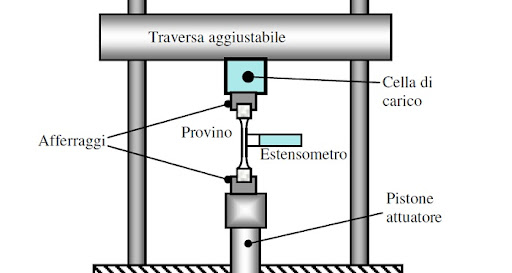
\includegraphics[width=10cm]{Proprietà_meccaniche/prova_trazione.jpg}
    \caption{Set up della prova di trazione}
    \label{fig:prova-trazione}
\end{figure}
La forma del provino è studiata in modo da ottimizzare il processo, la forma ad "osso di cane" permette di evitare la rottura in punti più sensibili come gli spigoli e favorire la rottura nella parte centrale dove il materiale è più omogeneo (il campo di forze non è omogeneo, al di fuori della zona centrale il bilanciamento delle forze non è più semplice).
Il risultato della prova di trazione dipende ovviamente dal materiale e dalle sue caratteristiche. In generale ciò che si misura è lo Stress (Forza/Area) in funzione dello Strain (Allungamento/Lunghezza del provino). Bisogna fare alcuni accorgimenti sulle definizioni che vengono utilizzate, in quanto né la sezione né la lunghezza del campione sono uguali durante il procedere della prova; se si considerano i valori uguali al valore iniziale allora si parla di \textbf{\textit{Engineering Stress e Engineering Strain}}, quando si fa riferimento ai valori istantanei si parla invece di \textbf{\textit{True Stress e True Strain}}. I grafici che si ottengono sono in genere differenti, solo per piccoli spostamenti si ha che queste due diverse quantità tendono allo stesso risultato:
$$\epsilon=\int_i^f\frac{dl}{l}=ln(l_f/l_i)=ln(l_i+\Delta l/l_i)\simeq\frac{\Delta l}{l_i}=\epsilon_{eng}$$
Non c'è da stupirsi di ciò in quanto il campione viene deformato e le lunghezze durante la prova cambiano.
\begin{figure}[h]
    \centering
    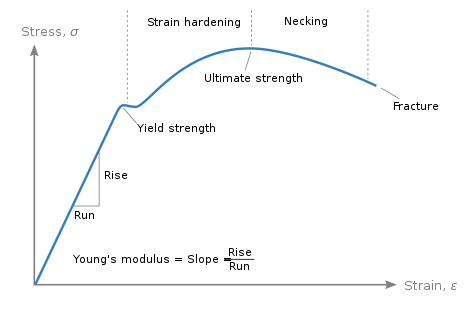
\includegraphics[width=10cm]{Proprietà_meccaniche/stress-strain.png}
    \caption{Stress-Strain curve}
    \label{stress-strain}
\end{figure}
In questi grafici è spesso possibile riconoscere tre zone differenti. Se guardiamo Fig \ref{stress-strain} possiamo vedere l'andamenteo dell'Engineering Stress in funzione dell'Engineering Strain:
\begin{itemize}
    \item In ogni grafico è presente una zona di \textbf{\textit{regime lineare o elastico}} in cui la deformazione è reversibile una volta tolto il carico; l'estensione di questa regione è legata all'intensità delle forze di legame.
    \item Arrivati ad un certo punto chiamato \textbf{\textit{punto di snervamento}} le deformazioni non sono più reversibili e si entra nel cosiddetto \textbf{\textit{regime plastico}}. A volte non è facile individuare questo punto, dunque si definisce per convenzione come punto di snervamento come il punto in cui permane una deformazione del 0.2\% del campione, per ritornare alla condizione iniziale occorre applicare una compressione il cui valore viene definita \textit{tensione residua}. In questo, una volta tolto il carico si ha che il campione non torna più allo stato iniziale ma vi rimane uno stress residuo.
    Non tutti i  materiali presentano questo regime: i materiali fragili si spezzano rimanendo in regime lineare. Il tipo  di rottura può essere duttile o fragile, a seconda della forma con cui si spezza il provino.
    \item Il grafico presenta un massimo detto \textbf{\textit{carico di rottura}}. Raggiunto questo punto si ha una deformazione su tutto il provino si inizia ad assistere al fenomeno di \textbf{\textit{strizione}} ed è considerato \textbf{\textit{failure}} ciò il materiale al di sopra di questo punto non può più essere impiegato. 
    \item Il punto in cui si ha la rottura del campione è detto \textbf{\textit{punto di rottura}}, il fatto che sia a valori più bassi è solo perché stiamo considerando le quantità ingegneristiche, se usassimo i valori reali avremmo una curva monotona crescente in quanto le dimensioni prese in considerazione diminuiscono nel corso della prova.
\end{itemize}
All'interno del regime lineare vale una legge del tipo:
\begin{equation}
    \sigma_{zz}=E\epsilon_{zz}
\end{equation}
$E$ è il modulo di Young ed è anche chiamata rigidezza, viene misurata in [kPa], [MPa] o [GPa]. Il modulo di Young in generale e diverso in base alla direzione ed al punto in cui si osserva, per materiali omogenei e isotropi possiamo ritenerlo costante. Se fossimo nel regime plastico potremmo definire un modulo di Young come: $\frac{d\sigma_{zz}}{d\epsilon_{zz}}$. 
Nel regime lineare, lo strain lungo z è collegato allo strain nelle altre direzioni:
\begin{equation}
    \nu=\frac{\sigma_{yy}}{\sigma_{zz}}=\frac{\sigma_{xx}}{\sigma_{zz}}
\end{equation}
$\nu$ viene chiamato modulo di Poisson è corrisponde alla contrazione della lunghezza trasversale rispetto allo strain; i valori di solito sono compresi tra 0 e 0,5 (per valori di 0,5 si ha la conservazione del volume). Valori inferiori allo 0 sono rari, ma non impossibili, e in questo caso significa durante la deformazione comporta un aumento del volume.
Vediamo ora alcune differenze tra le grandezze reali ed ingegneristiche.
Supponiamo di essere nel regime plastico in cui si ha conservazione del volume, cioè $A_0\cdot l_0=A\cdot l$
Si ha che:
$$\sigma_{eng}=\frac{F}{A_0}=\frac{F}{A}\cdot\frac{l_0}{l}=\sigma\cdot\frac{l}{l_0}$$
$$\epsilon=\int_i^f \frac{dl}{l}=ln(\frac{l_f}{l_i}=ln(\epsilon_{eng}+1)$$
Sopra abbiamo assunto che il materiale sia isotropo, ma in generale questa cosa non è vera e dovremmo avere rapporti di Possion diversi in direzioni diverse.
Con la prova di trazione è possibile ottenere moltissime informazioni, ma non è esaustiva per determinare tutte le proprietà meccaniche del provino; come vedremo più avanti esistono altre prove per misurare, ad esempio, la resistenza a compressione, flessione e torsione.
La resilienza è l'energia assorbita durante il processo in regime elastico, e corrisponde all'area sottostante al grafico (ha le dimensioni di un lavoro per unità di volume), mentre l'area sottesa da tutto il grafico viene definita tenacità; per materiali non isotropi entrambe dipendono dalla direzione in cui si effettua la prova.
$\sigma_{max}$ ci dà informazioni sulla resistenza; in generale per sistemi non omogenei e non isotropi può non essere ben definita in quanto dipende dalla direzione e da come viene effettuata la prova. Il modulo di Young ci dice quanto è rigido un materiale mentre $\epsilon_R$ riguarda la duttilità.
\begin{table}[h]
\centering
\begin{tabular}{@{}llcc@{}}
\toprule
\textbf{Materiale} & \textbf{Descrizione} & \textbf{Resistenza ($MPa$)} & \textbf{Modulo di Young ($GPa$)} \\ \midrule
PET  & Plastica termoplastica & 55 - 75 & 2 - 4 \\
Acciaio (AISI 304) & Acciaio inossidabile austenitico & 210 - 550 & 190 - 210 \\
Alluminio (Al 6061) & Lega di alluminio & 240 - 310 & 68 - 70 \\
Rame (Cu) & Metallo non ferroso & 110 - 220 & 110 - 130 \\
Legno (Pino) & Materiale naturale & 40 - 80 & 10 - 15 \\ \bottomrule
\end{tabular}
\caption{Proprietà meccaniche di alcuni materiali}
\label{tab:proprietà_materiali}
\end{table}


\begin{wrapfigure}{l}{0.43\textwidth}[h]
  \centering
  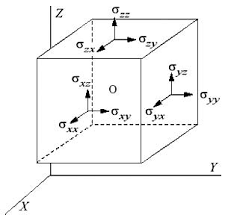
\includegraphics[width=0.26\textwidth]{Proprietà_meccaniche/cubetto.png}
  \caption{cubetto}
  \label{cubetto}
\end{wrapfigure}

Per capire come si comporta macroscopicamente il materiale andremo a vedere come agiscono le tensioni su di un cubetto di dimensioni infinitesime dXdYdZ (Fig \ref{cubetto}): definiamo il tensore degli sforzi: $$\sigma_{ij}$$ dove i indica direzione della normale alla faccia e j invece indica la direzione della forza.
In generale è possibile dimostrare che questo tensore è simmetrico (e quindi anche diagonalizzabile), in caso contrario è possibile dimostrare che esiste un momento torcente non nullo sul nostro cubetto che ne causerebbe la rotazione.
In molti casi pratici si cerca di ricondursi a stress mono- o biassiale, che algebricamente significa ridurre il tensore degli sforzi ad un solo autovalore (condizioni monoassiali) o due autovalori (condizioni biassiali) nonnulli; questo ad esempio è il caso della prova di trazione di materiali omogenei ed isotropi. \textcolor{red}{chiedere a Milazzo come cambia la prova di trazione per materiali inomogenei e anisotropi}. Al tensore degli sforzi è associato un tensore delle deformazioni $\epsilon_{ij}$; in generale la relazione che c'è tra i due è sempre un'applicazione lineare simmetrica ma non è banale (lineare quando ci troviamo nel regime elestico ovviamente). In generale si ha una relazione del tipo:
\begin{equation}
    \sigma_{ij}=E_{ijkl}\epsilon_{kl}
\end{equation}

\subsection{Prova di flessione}

\begin{figure}[h]
    \centering
    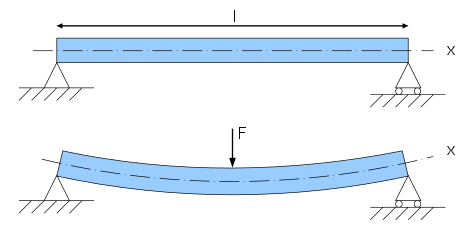
\includegraphics[width=10cm]{Proprietà_meccaniche/prova-flessione.png}
    \caption{Set up della prova di flessione a tre punti, esistono set up in cui sono presenti quattro punti differenti; la dinamica è differente in quanto lo stress subito dai vari punti è differente.}
    \label{fig:prova-flessione}
\end{figure}

La prova di flessione, mostrata in figura \ref{fig:prova-flessione}, consiste nell'applicazione di un provino di forma allungata tre o quattro forze con risultante nulla (si parla rispettivamente di prova a tre o a quattro punti) in punti differenti e su lati opposti del campione. In questo modo non si produce una forza complessiva sul provino, ma viene generato un momento torcente, pertanto alcune zone del materiale sono sottoposte a trazione mentre altre sono sottoposte a compressione. Chiamiamo \textit{fibre} le linee parallele ai due del provino che sono sottoposti a forze; esiste sempre una fibra, detta \textbf{\textit{fibra neutra}}, per cui vale $\sigma_{zz}=0$; tipicamente questa passa per il baricentro del provino, ma vedremo tra poco un'importante eccezione. In generale, soprattutto se il provino non è omogeneo, sapere dove si trova la fibra neutra è importante in quanto i punti più distanti dalla fibra neutra sono quelli in cui si verifica cedimento più facilmente.
Nel caso illustrato in Fig \ref{fig:prova-flessione} vale la legge:
\begin{equation}
    \sigma_x(z)=\frac{M_y}{J_y}z
\end{equation}
Dove $M_y$ è il momento delle forze, $J_y$ è il momento d'inerzia nel piano $xz$ e $z$ è la coordinata nel piano ortogonale alla fibra baricentrica.
Nel regime lineare vale che i contributi si sommano semplicemente, dunque la formula più generale possibile per un corpo sottoposto a flessione su due lati con una trazione (o compressione, più comune soprattutto in ingegneria civile) è:
\begin{equation}
    \sigma_{zz}=\frac{M_x}{J_x}y-\frac{M_y}{J_y}x+F
\end{equation}
dove $F$ è appunto la forza di trazione o compressione. Dal momento che la fibra neutra è quella in cui lo stress è nullo la presenza della forza costante sposta la fibra neutra del baricentro. In generale è possibile osservare che le figure cave come tubi presentano resistenze alle flessioni maggiori in quanto sono quelle che hanno momento d'inerzia maggiore, e questa è una delle ragioni per cui le travi vengono realizzate con forma a doppia T e non sono piene.

\begin{figure}[h]
    \centering
    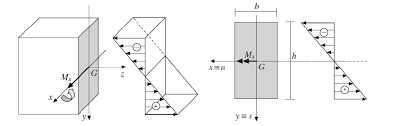
\includegraphics[width=10cm]{Proprietà_meccaniche/fibra neutra.png}
    \caption{Stress percepito da punti in posizioni differenti lungo il campione. La presenza di una forza ha l'azione di traslare il baricentro.}
    \label{fibra-neutra}
\end{figure}

Il test di flessione trova impiego, ad esempio, per la misura delle proprietà dei ceramici. Preparare i campioni dei materiali ceramici per il testi di trazione con le forme adeguate (senza spigoli) non è facile, inoltre anche creare il grip e fissarlo alla macchina senza causare crepe è una cosa non scontata. 
Inoltre si spezzano a valori molto piccoli (0.1\%) e richiede che il campione sia perfettamente allineato senza che esistano stati di flessione in quanto falsano la prova. Il bending test elimina questi problema in quanto la frattura avviene comunque nel lato di trazione.

\subsection{Prova di torsione}

La prova di torsione è tendenzialmente la più complessa da descrivere matematicamente, dato che le equazioni dipendono dalla forma del provino.
Supponiamo di effettuare la prova di torsioni di un cilindro, che è un caso abbastanza comune e semplice. In questo caso la prova di torsione tipica (Fig \ref{prova di torsione}) consiste nel fissare un'estremità mentre all'altra viene applicata un momento torcente.

\begin{figure}[h]
    \centering
    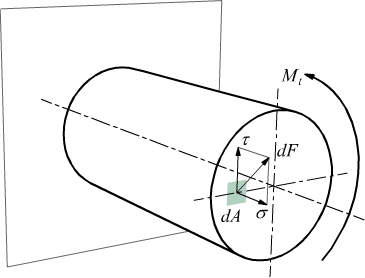
\includegraphics[width=8cm]{Proprietà_meccaniche/provaditorsionemetalli.png}
    \caption{Prova di torsione.}
    \label{prova di torsione}
\end{figure}

In generale la torsione è molto complicata, è possibile farla in maniera semplice solo in alcuni casi ad alta simmetria come la torsione in un cilindro.
La relazione in questo caso è simile alla flessione:
\begin{equation}
    \tau=G\theta
\end{equation}
G che è lo shearing elastic module dipende dalla forma del campione. Nel caso mostrato in figura si ha che:
\begin{equation}
    \tau_{yz}=\frac{M_z}{J_z}r
\end{equation}
Dove $J_z$ è il secondo momento d'inerzia, r è il raggio del cilindro. In ogni caso G non è indipendente da E e da $\nu$ ma nel caso di materiali isotropi ed omogenei vale:
\begin{equation}
    E=2G(1+\nu)
\end{equation}
Per motivi energetici $\nu$ (\textbf{\textit{modulo di Poisson}}) è quasi sempre compreso tra -1 e 1/2.



\subsection{Prove di durezza}
Le prove di durezza consistono nell'osservare la capacità di un materiale nel non essere penetrato da un altro. Esistono diverse prove di durezza:
\begin{itemize}
    \item \textbf{\textit{Brinnel}}: in questa prova si utilizzano delle sfere di materiale duro (WC) con un certo raggio R che vengono pressate sul nostro campione in modo da creare una deformazione permanente (è un test distruttivo ovviamente).
    \begin{equation}
        HB=\frac{F}{\pi 2R P}
    \end{equation}
    F è la forza impressa sulla sfera, P è la profondità con cui penetra il nostro campione; da notare che anche se le dimensioni di HB sono una pressione, questa non ha un vero senso fisico.
    Ovviamente è possibile misurare solo campioni con una durezza minore di WC. La dimensione della sfera è scelta in base la dimensione del campione in quanto misure effettuate con campioni con spessore differente non sono comparabili. Un altra cosa a cui stare attenti è quando si usano materiali troppo morbidi in cui la sfera può completamente entrare, di solito si segue la regola che 0.25<d/D<0.5 dove d è il diametro dell'impronta e D il diametro della sfera. Per confrontare test effettuati con sfere la cui dimensione è diversa di solito si osserva l'angolo, i protocolli più validi sono quelli che lasciano l'angolo uguale in prove differenti.
    
    \item \textbf{\textit{Vickers}}: il test Vickers utilizza invece una punta a forma di prisma (presenta un angolo di 136°) e lavora in microscale andando a misurare la penetrazione (il test può essere considerato non distruttivo).
    \begin{equation}
        HV=\frac{F}{d^2}K
    \end{equation}
    K è un coefficiente numerico (vale 1.854), d è la diagonale del quadrato impresso dal prisma. Questo metodo presenta alcuni problemi, se il materiale è molto morbido la forma impressa potrà essere di difficile interpretazione, inoltre è un metodo molto costoso.
    \item \textbf{\textit{Rockwell}}: in questo test si usa una punta conica con un angolo di 120° in cui sono presenti delle tacche equidistanziate. La durezza è data dal numero di tacche che riescono a penetrare il materiale. Il valore della durezza è dato da:
    \begin{equation}
        HR=100-x
    \end{equation}
    x è il numero di tacche. La presenza di tacche permette calibrazioni
    \end{itemize}
Le relazioni tra test differenti sono difficili, grossolanamente è possibile dire: HR$\simeq$3HB. Nel test Vickers siamo vicini al punto di snervamento (la deformazione è molto piccola), le altre lavorano nel regime plastico.

\subsection{Toughness test}
\begin{figure}[h]
    \centering
    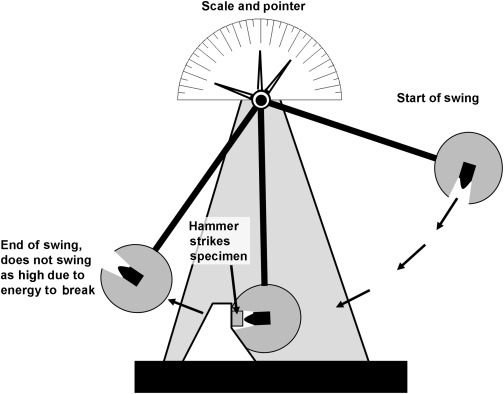
\includegraphics[width=8cm]{Proprietà_meccaniche/toughnesstest.jpg}
    \caption{Toughness test.}
    \label{oughnesstest}
\end{figure}

Il test di tenacità misura la quantità di energia che il materiale riesce ad assorbire prima della rottura. 
In realtà il test di trazione permette di ottenere informazioni sulla tenacità del nostro materiale, spesso però non è sufficiente in quanto le condizioni in cui viene effettuato il test sono fin troppo ideali (situazione di stress uniassiale). In questo test (Fig \ref{oughnesstest}) la forma del campione è diversa in modo da favorire la rottura in un punto specifico. Il principio è rilasciare un peso e misurare l'energia assorbita dal campione nel processo di rottura misurando la differenza di energia potenziale del pendolo.
Ogni test ha una forte dipendenza dalla temperatura, questo è dovuto al fatto che in molti materiali all'aumentare della temperatura si ha un aumento dell'allungamento massimo prima della rottura (il materiale diventa progressivamente più duttile). La cosa molto interessante è che non si ha un aumento lineare con T ma con forma sigmoidale. Il punto d'inversione della derivata seconda è anche detto temperatura di transizione duttile fragile.
Non tutte le strutture presentano questa transizione ed alcune sono più favorite rispetto ad altre come in Fig \ref{duttile-fragile} (\textcolor{red}{chiedere a milazzo perche si ha questo solo per BCC e non FCC}.
\begin{figure}[h]
    \centering
    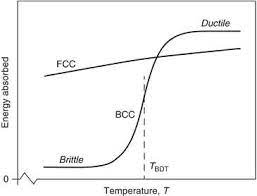
\includegraphics[width=6cm]{Proprietà_meccaniche/duttile-fragile.jpg}
    \caption{Grafico in cui è illustrata una transizione duttile-fragile.}
    \label{duttile-fragile}
\end{figure}

\newpage
\section{Struttura}

\epigraph{Direzioni cristallografiche |u v w| dove sono numeri interi, è come un vettore normale i cui vettori di base sono quelli primitivi}{\textit{Leonardo Sabattini}, I edizione}

Possiamo raggruppare i solidi in tre gruppi principali:
\begin{itemize}
    \item Cristallini.
    \item Amorfi.
    \item Parzialmente cristallini.
\end{itemize}
Le strutture ordinate si ottengono grazie alle interazioni elettrostatiche che si creano (legami covalenti, metallici, interazioni dipolo-dipolo). Al di sotto di una certa temperatura queste interazioni vincono i moti termici e, nel caso di atomi, questi si organizzano in un \textbf{\textit{reticolo cristallino}}, strutture periodiche ordinate definite da 3 vettori \textbf{\textit{primitivi}} a partire dai quali è possibile generare tutto il reticolo. In generale in ogni punto del reticolo possono trovarsi uno o più atomi; poiché non è sempre possibile individuare tutti i punti del reticolo partendo da un solo punto del reticolo in alcune strutture è necessario definire una base costituita da più punti; il caso più semplice sono i monocristalli.
L'organizzazione spaziale degli atomi in 3D rispetta uno dei 14 reticoli di Bravais (230 gruppi spaziali se si aggiungono anche le simmetrie). Non tutti reticoli cristallini hanno la stessa efficienza nell'impacchettare gli atomi: più compatti sono l'FCC (face centered cubic) ed l'HCP (Hexagonal close packed), entrambi hanno un atomic packing factor di 0,74 (entrambi sono ottenuti allo stesso modo ma posizionando le sfere in maniera sfalsata). Sapere la struttura cristallina è molto importante in quanto molte proprietà dei materiali dipendono da essa.
Definiamo alcune cose che possono essere utili:
\begin{itemize}
    \item Direzioni cristallografiche |u v w| dove sono numeri interi, è come un vettore normale i cui vettori di base sono quelli primitivi; con <u v w> si indica una famiglia (sono caratterizzati dalla stessa distanza atomica: |1 0 0|, |0 1 0|, ...).
    \item Piani cristallini (h k l), le lettere indicano le celle in cui il piano si interseca; una famiglia di piani è definita come \{ h k l \} (piani distanziati ma paralleli).
\end{itemize}
In generale è importante sapere quali piani cristallini e quali direzioni presentano la massima densità in quanto alcuni processi dipendono da esso. Un'altra cosa importante che è associata alla struttura cristallina sono i suoi \textbf{\textit{siti interstiziali}}. Sono importanti in quanto artefici della diffusione di altre specie all'interno di un materiale. Il rapporto tra i raggi della specie che si vuole aggiungere al cristallo e quello già presente determina il tipo di interstizio ed il numero di coordinazione della specie: se il rapporto è piccolo si occuperà una cavità tetraedrico, all'aumentare delle dimensioni si avrà coordinazione ottaedrica e, per raggi molto simili, anche strutture cubiche.\\
In generale non si ha mai un cristallo unico ma si lavora con un materiale policristallino, formato cioè da molti cristalli più piccoli detti \textbf{\textit{grani}}, sono separati tra loro da \textbf{\textit{bordi di grano}}. In generale però si possono avere anche strutture non ordinate, ad esempio quando il raffreddamento dalla fase liquida è talmente veloce da bloccare la diffusione ed impedire la riorganizzazione in un reticolo cristallino. Si ottiene allora un sistema metastabile e tendenzialmente una struttura amorfa. Alcuni polimeri possono raggiungere un grado di cristallinità elevato mantenendo comunque un certo grado di disordine.

    \begin{figure}[h]
    \centering
  \begin{minipage}[b]{0.3\linewidth}
    \centering
    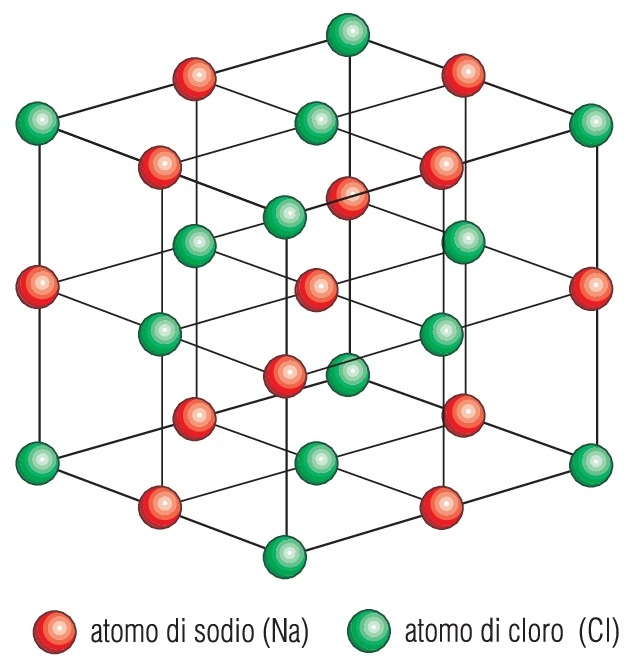
\includegraphics[width=\linewidth]{struttura/cristallo.jpg}
    \label{cristallo}
  \end{minipage}
  \begin{minipage}[b]{0.3\linewidth}
    \centering
    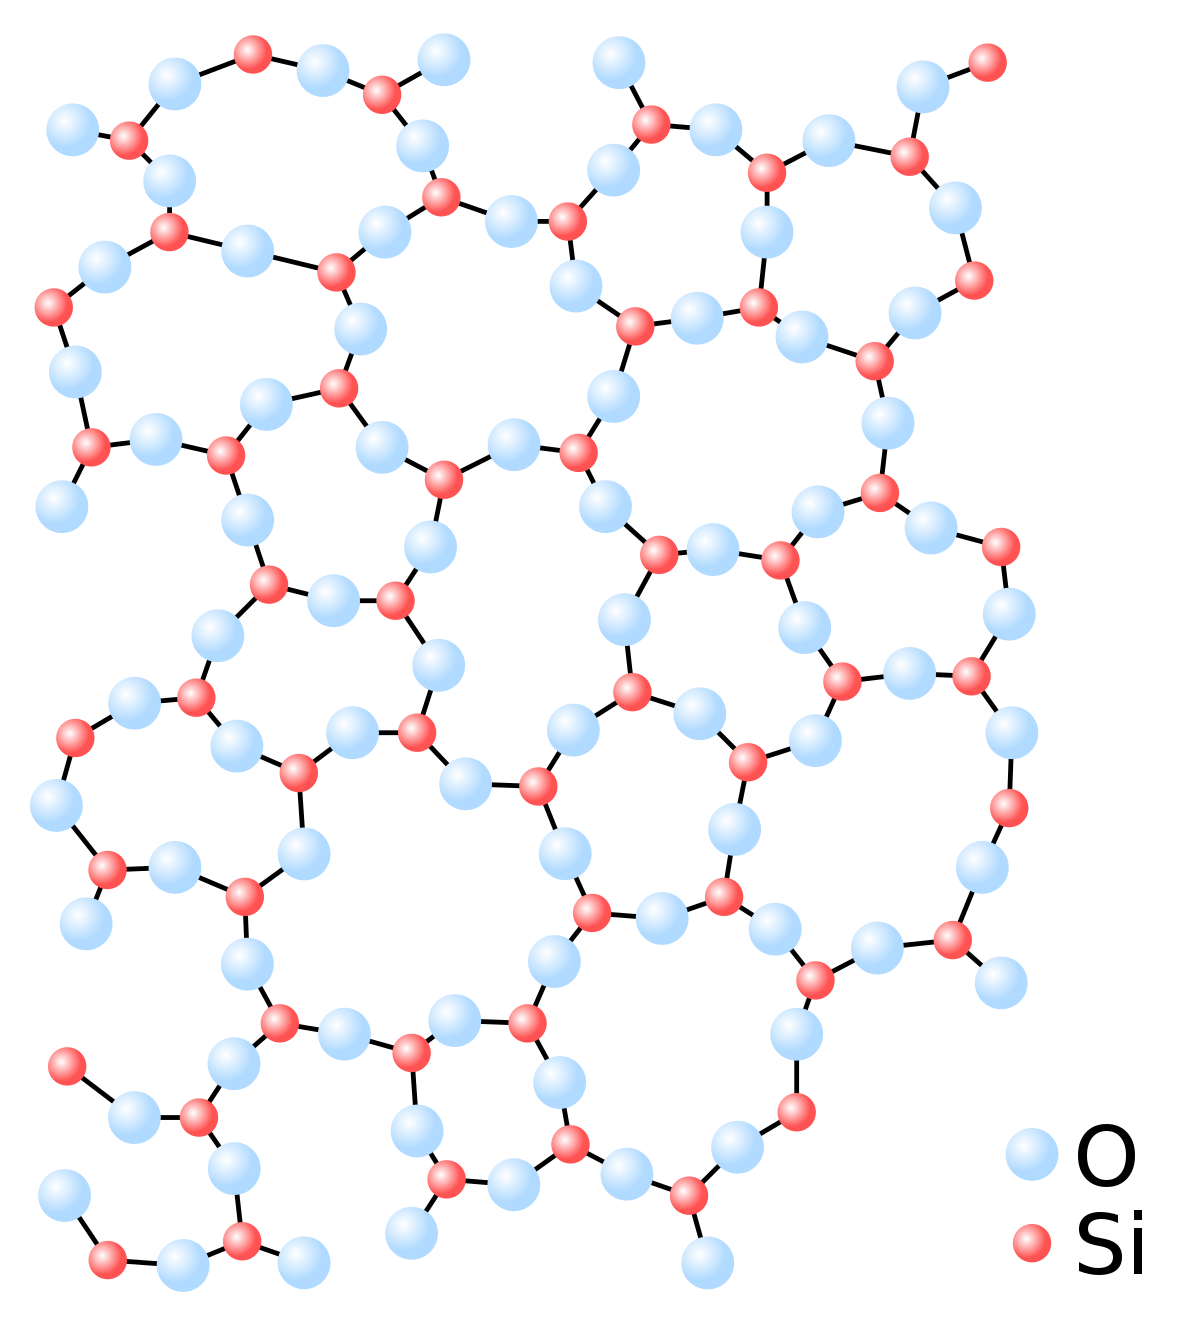
\includegraphics[width=\linewidth]{struttura/amorfo.png}
    \label{amorfo}  

  \end{minipage}
    \begin{minipage}[b]{0.3\linewidth}
    \centering
    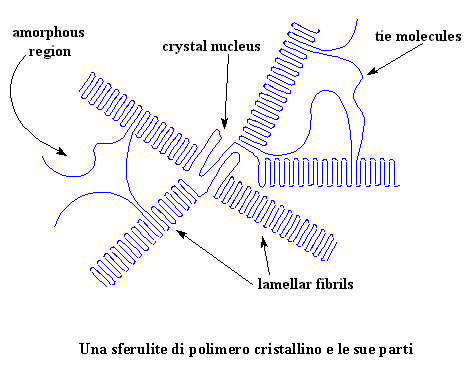
\includegraphics[width=\linewidth]{struttura/polimero,semicristallino.jpg}
    \label{semi}  

  \end{minipage}

  \caption{Sinistra: cristallo, struttura amorfa, struttura semicristallina.}
  
\end{figure}

\subsection{Solidificazione dei metalli}
La solidificazione avviene ovviamente per motivi termodinamici ovvero quando l'energia libera della forma solida è uguale a quella della fase liquida. In generale la pendenza (rappresentata dall'entropia) della fase liquida è maggiore di quella della fase solida, e quindi a T più alta la prima risulta più stabile.
All'equilibrio si ha:
\begin{equation}
    \Delta G_V=G_s-G_v=0
\end{equation}
Se la temperatura diminuisce la fase solida diventa più favorita ed il contributo è sempre negativo; bisogna però considerare bene questo processo in si crea un'interfaccia tra le due fase. Una descrizione quantitativa di questo fenomeno richiede l'introduzione della tensione superficiale:
\begin{equation}
    \Delta G_T=\frac{4}{3}\pi r^3\Delta G_V+\gamma\pi r^2
\end{equation}
dove $\gamma$ è la tensione superficiale ed è sempre positiva. La nucleazione e l'eventuale formazione di cristalli possono avvenire solo se si riesce a superare una certa dimensione critica:
\begin{equation}
    r^*=-\frac{2\gamma}{\Delta G_v}=-\frac{2\gamma T_m}{\Delta H_v(T_m-T)}
\end{equation} 
Questa dimensione deve essere la minore possibile in quanto l'energia massima del processo dipende da questa quantità (anche $\gamma$ dovrebbe essere una funzione di T in realtà).
Il valore del raggio critico definisce il rate di creazione di questi cristalli:
\begin{equation}
    v_d=K_1\exp(-\frac{\Delta G*}{kT}
\end{equation}
Un altro processo che entra in gioco è la diffusione:
\begin{equation}
    v_d=K_2\exp\left(-\frac{Q_d}{KT}\right)
\end{equation}
Questo processo di cristallizzazione è detto \textbf{\textit{omogenea}}.
Spesso la cristallizzazione avviene però in maniera \textbf{\textit{eterogenea}}, sfruttando cioè la presenza di superfici o di cristalli già esistenti; in questo caso è più facile ottenere un raggio di curvatura maggiore del raggio critico. Inoltre, questo metodo richiede temperature di sottoraffreddamento minori.

\subsection{Microstrutture}

\epigraph{sono i primi a formarsi a causa delle superfici fredde della forma}{\textit{Leonardo Sabattini}, I edizione}

La struttura di grano dipende molto da come il materiale è stato raffreddato ed è importante per capire le proprietà meccaniche di un oggetto. Materiali che presentano strutture di grano sottili sono in genere più resistenti a temperature basse, mentre il comportamento si inverte quando si lavora ad alte temperature, ed è quindi preferito lavorare con monocristalli.
\begin{figure}[h]
    \centering
    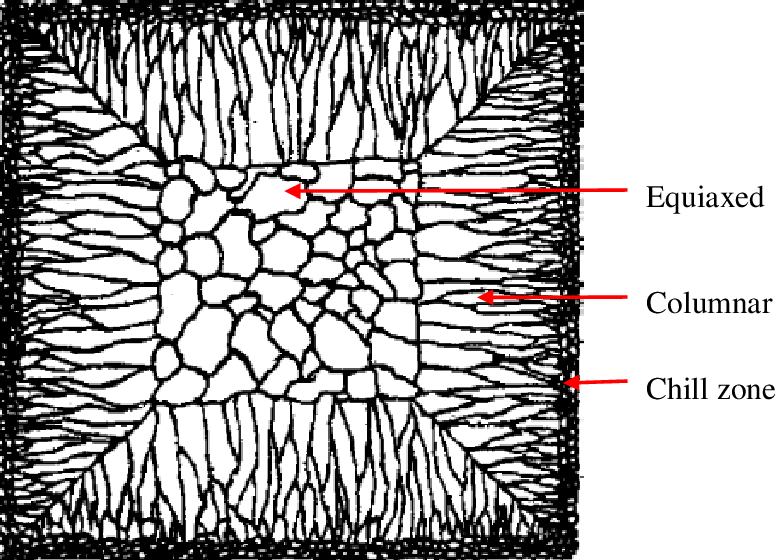
\includegraphics[width=6cm]{struttura/colata_grain.png}
    \caption{Struttura di grano.}
    \label{colata}
\end{figure}
In generale durante la colata si generano grani di dimensione differente (rappresentati in Fig \ref{colata}):
\begin{itemize}
    \item Chill zone: sono i primi a formarsi e si trovano lungo la superficie dello stampo, nella regione che si raffredda per prima. \textcolor{red}{DA RICONTROLLARE hanno dimensioni piccole e forma irregolare; da loro dipende la durezza del manufatto}
    \item Columnar zone: la forma di questi grani è associata ai moti convettivi e al modo in cui il calore fluisce dal centro del campione verso l'esterno, pertanto sono allungati ed ortogonali alle pareti dello stampo.
    \item Equiaxial zone: hanno nuovamente una dimensione piccola, sono dovuti alla presenza di elementi di lega od in generale alla presenza di altre specie come raffinatori di grano, di solito hanno una forma tonda ed un orientazione randomica.
\end{itemize}
Per ottenere grani più piccoli vengono usati i cosiddetti \textbf{\textit{raffinatori di grano}}. La colata su di una forma non è l'unico modo di lavorazione, altri metodi procedono per colata continua (ad esempio quelli utilizzati per la produzione dell'acciaio).
Se vogliamo ottenere invece monocristalli è necessario ricorrere ad altre tecniche specifiche; ad esempio si può usare il processo "pigtail" in cui si usa uno strumento a forma di coda di maiale che permette l'eliminazione e la crescita selettiva di cristalli con una particolare orientazione (questo metodo è impiegato per produrre turbine monocristalline che lavorano ad alta T). Un altro metodo visto a lezione sfrutta un singolo cristallo già esistente che funge da seme, permettendone l'accrescimento tramite opportuna modulazione della temperatura e delle condizioni di lavoro. Affinché il processo venga bene, infatti, il liquido in contatto con il cristallo deve essere ad una temperatura molto vicina a quella di fusione instaurando un equilibrio (con questo metodo viene sintetizzato il silicio monocristallino). Ovviamente i metodi usati per produrre materiali monocristallini sono generalmente più costosi degli altri.

\section{Imperfezioni}

\epigraph{I due tipi più sono: a vite o a spigolo o miste.}{\textit{Leonardo Sabattini}, I edizione}

Ci sono diversi tipi tipi di imperfezioni nei cristalli con una conseguente perdita di periodicità. Non tutti i difetti sono accidentali, spesso si aggiungono di proposito come accade col drogaggio dei semiconduttori.
Le imperfezioni sono classificate in base alla dimensionalità:
\begin{itemize}
    \item \textbf{\textit{Difetti puntuali (0D)}}: sono di vario tipo: interstiziali, quando si ha una specie estranea all'interno degli spazi vuoti del reticolo, oppure sostituzionali, quando la specie è sostituita con un altro elemento. 
    Un altro tipo di imperfezioni sono rappresentate dalle vacanze, ovvero posizioni cristalline in cui si ha l'assenza di un atomo; questo può essere dovuto ad esempio a vari processi durante il processo di raffreddamento. 
    Questi difetti creano delle tensioni che coinvolgono le immediate vicinanze ma che tendono a scomparire a grandi distanze.
    In aggiunta, nei solidi ionici abbiamo:
    \begin{enumerate}
        \item Difetti di Frenkel, dove uno ione è spostato dalla sua posizione nel reticolo e occupa una posizione interstiziale.
        \item Difetti di Schottky, dove si ha una vacanza sia di un catione che di un anione (per preservare l'elettroneutralità).
    \end{enumerate}
    L'origine dei difetti puntuali (mostrati in fig. \ref{defects}) può essere di varia natura, ad esempio potrebbe essere dovuto al processo di raffreddamento troppo veloce che non permette il raggiungimento dell'equilibrio, in ogni caso la loro presenza comporta sicuramente un aumento dell'entropia. La frazione di siti difettati (Shottky o Frenkel) può essere stimato usando la legge di Boltzmann:
    \begin{equation}
        \chi_{dif}=\exp\left(-\frac{E_{dif}}{KT}\right)
    \end{equation}
    La legge scritta sopra è valida solo in condizioni di equilibrio.
    \begin{figure}[h]
        \centering
        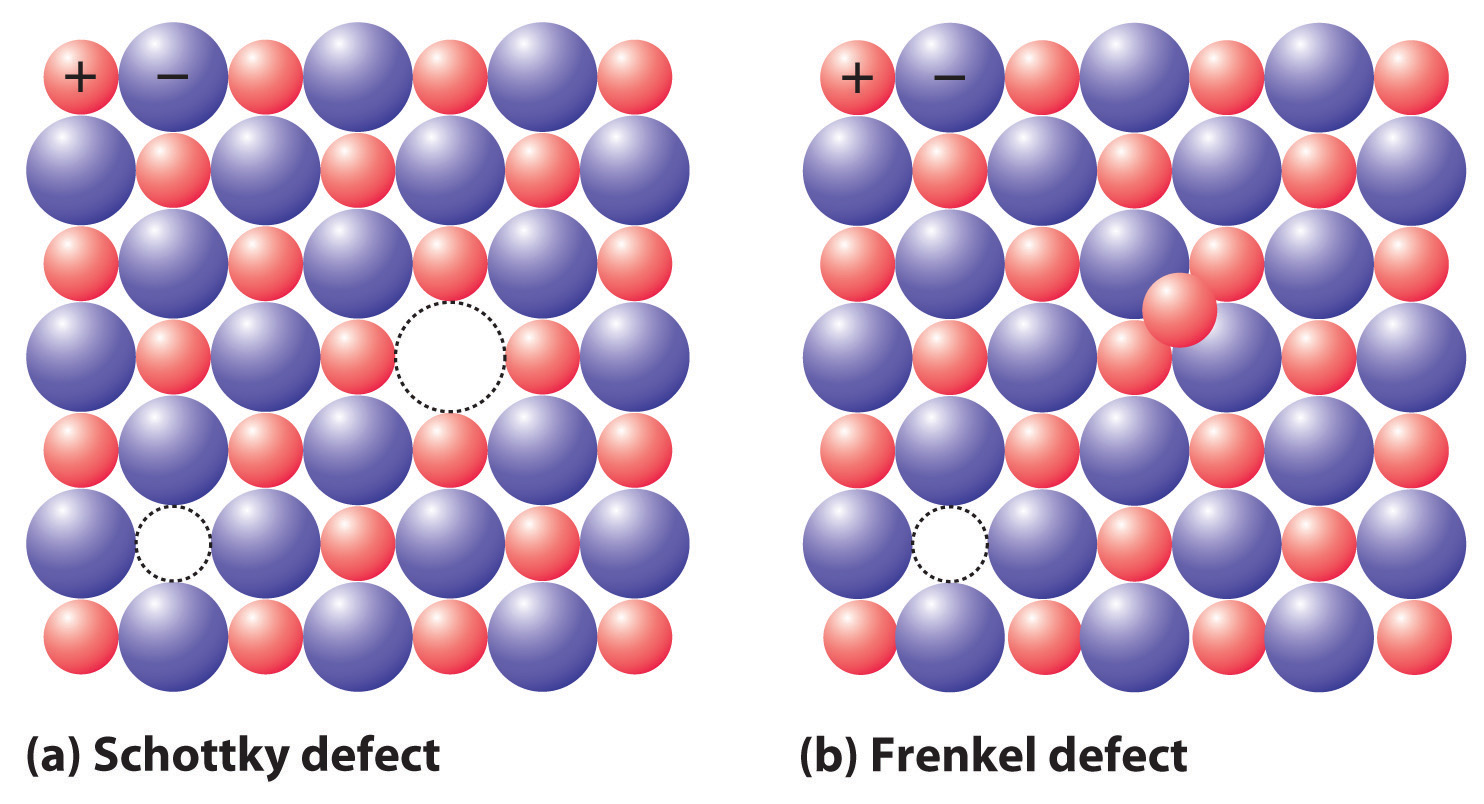
\includegraphics[width=5cm]{struttura/shottky.jpg}
        \caption{Tipi di dislocazioni puntuali: sinistra è di tipo Shottky, destra è di tipo Frenkel.}
        \label{defects}
    \end{figure}
    \item \textbf{\textit{Difetti 1D}}: vengono anche chiamate dislocazioni, e sono determinanti in molti processi e fenomeni che determinano le proprietà meccaniche dei materiali, soprattutto la plasticità. I due tipi di dislocazioni che individuiamo sono quelle a vite e quelle a spigolo; esistono anche le dislocazioni miste che sono una combinazione delle due tipologie precedenti. Possono essere dovute a deformazioni plastiche che inducono lo spostamento di filari di atomi, ma anche a raggruppamento di vacanze. La natura della dislocazione viene definita dal vettore di Burgers: la direzione è perpendicolare alla dislocazione mentre il modulo è uguale alla distanza rispetto alla posizione di equilibrio.
        \begin{figure}[h]
    \centering
  \begin{minipage}[b]{0.4\linewidth}
    \centering
    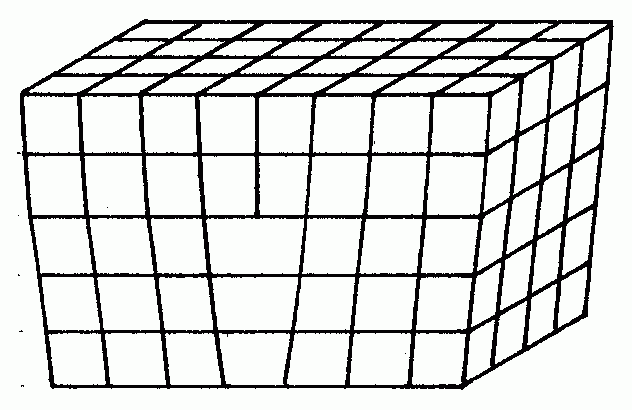
\includegraphics[width=\linewidth]{struttura/screw_dislo.png}
    \label{screw}
  \end{minipage}
  \begin{minipage}[b]{0.4\linewidth}
    \centering
    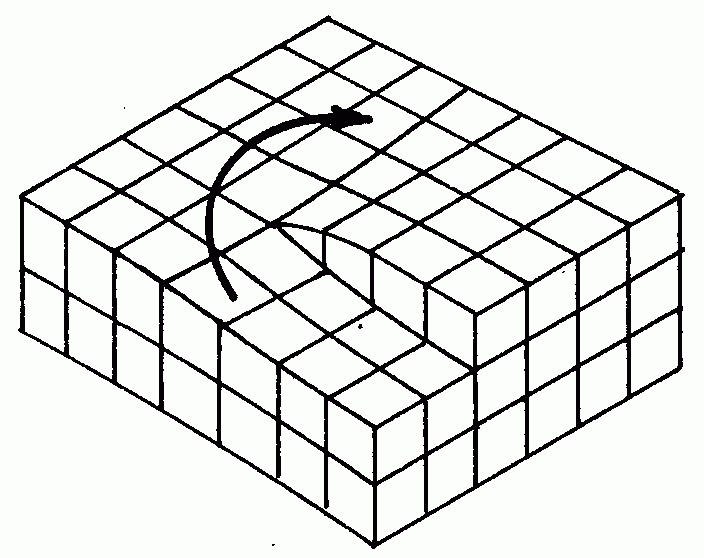
\includegraphics[width=\linewidth]{struttura/Dislocation_hélicoïdale.png}
    \label{dislo}  

  \end{minipage}
  \caption{Sinistra: dislocazione a spigolo, destra: a vite}
\end{figure}
    \item \textbf{\textit{Difetti di superficie}}: i difetti di superficie più frequentemente incontrati sono i bordi di grano. Nei bordi di grano si raggruppano le imperfezioni e spesso agiscono come centri di nucleazione. Altri difetti bidimensionali sono gli stacking e il twinning. I bordi di grano sono zone in cui due monocristalli, generalmente con orientazione differente, si incontrano, e tipicamente hanno uno spessore pari a qualche passo reticolare.
    \item \textbf{\textit{Difetti di volume}}: lo si ha quando diversi difetti puntuali si raggruppano.
\end{itemize}

\subsection{Diffusione nei solidi}

\epigraph{Deformazioni plastiche+come avvengono deformazioni e come sono involuite le dislocazioni}{Sun Tzu, \textit{l'arte della guerra [contro la lingua italiana, ndr]}}

Il processo di diffusione avviene tanto nei liquidi quanto nei solidi. Affinché la diffusione avvenga è necessario superare un'energia di attivazionem in quanto essa segue una cinetica di tipo Arrhenius. 
La diffusione si ha principalmente nei solidi con difetti sostituzionali e interstiziali. La velocità di diffusione dipende dall'energia che a sua volta dipende dalla natura dal reticolo cristallino e dalla natura della specie che diffonde: si osserva che nei solidi con difetti interstiziali è più bassa rispetto a quelli sostituzionali; per dare ordini di grandezza, se le prime sono sui 10 kcal/mol, le seconde stanno sopra i 50 kcal/mol.
Alcuni esempi che utilizzano la diffusione nei solidi sono la precipitazione di solidi (la creazione di leghe), il moto dei difetti e la nucleazione di nuovi grani. 

La diffusione allo stato stazionario segue la legge di Fick:
\begin{equation}
    J(x)=-D\frac{\partial C(x)}{\partial x}
\end{equation}
Dove $J$ è il flusso su una superficie e $D$ è la diffusività [m/s$^2$]. D dipende da tanti fattori:
\begin{itemize}
    \item Dalla struttura cristallina.
    \item Dalla temperatura.
    \item Dalla concentrazione di soluto.
    \item Dalla presenza di difetti.
\end{itemize}.
In condizioni non stazionarie si segue invece la seconda legge di Fick:
\begin{equation}
    \frac{\partial C(x,t)}{\partial t}=\frac{\partial }{\partial x}\left(-D\frac{\partial C(x)}{\partial x}\right)
\end{equation}
Sapere come si comporta la diffusione è importante in quanto diversi processi industriali ne fanno utilizzo come la carburazione dell'acciaio, il doping dei semiconduttori e la sinterizzazione delle ceramiche. Nei materiali ceramici dove sono presenti legami ionici la situazione è più complessa, in quanto l'elettroneutralità va conservata e quindi i processi diffusivi di specie cariche coinvolgono sempre almeno due specie differenti, limitando la diffusione alla specie più lenta.
Le deformazioni avvengono nei piani con la maggiore densità atomica e lungo le direzioni con la maggiore densità lineare.
Nei cristalli ionici le cose sono più complicate in quanto fatto da ioni di carica opposta: lo scorrimento può avvenire lungo la direzione che non implica la sovrapposizione di atomi con lo stesso segno.
Twinning and shear force (avviene meglio per HCP: struttura rombica, sensato). 

\subsection{Meccanismi d'indurimento e rafforzamento}

Esistono diversi metodi di rafforzare un manufatto. In generale si cerca di agire su difetti e dislocazioni in modo da ostacolarne la propagazione e quindi aumentare la rigidezza del campione; un'altra soluzione, impraticabile il più delle volte, consiste nel creare monocristalli perfetti.

\begin{itemize}
    \item Creazione di soluzioni solide
    \item precipitazioni di nanofasi
    \item Rafforzamento dei bordi di grano
    \item Incrudimento.
\end{itemize}

\subsection{Soluzioni solide e precipitazione di nanofasi}

I metalli puri presentano piccoli valori di snervamento, per questo viene aggiunto un secondo elemento (nelle soluzioni solide) o una seconda fase per migliorarne le proprietà meccaniche.
Nelle soluzioni solide viene sostituito parzialmente il nostro elemento con un'altra specie con dimensioni differenti che andranno ad aumentare il numero di dislocazioni aumentandone la rigidezza senza però modificare in maniera sostanziale altre proprietà.
Nell'incrudimento per precipitazione invece si crea proprio una nuova fase che andrà a limitare ancora di più il movimento delle dislocazioni. Più queste nanofasi saranno piccole e finemente disperse maggiore sarà l'ostacolo.
Nelle \textbf{\textit{leghe di metalliche}} si crea un miscuglio omogeneo tra il nostro elemento iniziale che funge da solvente ed elementi esterni, chiamati elementi di lega, che fungono da soluti. In generale possiamo avere  \textbf{\textit{substitutional solid solutions}} or  \textbf{\textit{interstitial solid solutions}}.
Le leghe metalliche di solito hanno proprietà simili al metallo iniziale con la differenza che le T$_m$ non è più precisa ma spesso è un intervallo; si parla quindi di \textbf{\textit{fusione incongruente}}.
Le soluzioni solide possono essere di più tipi:
\begin{itemize}
    \item  \textbf{\textit{primario}} se la struttura cristallina viene mantenuta.
    \item  \textbf{\textit{secondario}} se la struttura cristallina della lega è differente da quella del metallo più abbondante (si verifica raramente).
    \item  \textbf{\textit{composti intermetallici}} se è un composto chimico vero e proprio con delle proporzioni precise. In questo caso non si ha più il tipico legame metallico ma spesso ha forte carattere covalente ed emergono proprietà differenti dai metalli soliti.
\end{itemize}
Perchè si formi una \textbf{\textit{soluzione solida sostituzionale}}(l'elemento di lega si va a sostituire al nostro elemento nel reticolo) empiricamente si è osservato che:
\begin{enumerate}
    \item I due elementi devono presentare dimensioni simili (raggio atomico differente al più del 15\%).
    \item Avere stesso reticolo cristallino.
    \item Avere simile elettronegatività.
    \item Avere stessa valenza.
\end{enumerate}
Queste regole sono dette regole di \textbf{\textit{Hume-Rothery}}. In caso di solubilità parziale empiricamente si osserva che l'elemento che ha maggiore valenza presenta una maggiore solubilità.
Per ottenere una \textbf{\textit{soluzione solida interstiziale}}, invece, le dimensioni del soluto devono essere minori di quelle del solvente e rispettare rapporti abbastanza stringenti; di solito solo O, B, H, C, N riescono a dare questo tipo di soluzioni.
In genere le soluzioni solide mantengono le proprietà metalliche diventando però più dure e resistenti a causa delle tensioni interne; le proprietà di trasporto però peggiorano.
La dimensione dell'elemento di lega influisce sulla tensione che genera alla struttura e quindi anche all'impatto che esso provoca al campione. Una piccola aggiunta di berillio aumenta molto la tensione di snervamento del rame rispetto allo zinco o al nichel che presentano dimensioni simili.

\subsection{Precipitation hardening}

La precipitazione avviene quando la variazione di energia libera è negativa:
\begin{equation}
    \Delta G_T=(\Delta G_{\alpha\rightarrow\beta}+\epsilon)\frac{4\pi r^3}{3}+4\pi \gamma r^2
\end{equation}
$\epsilon$ rappresenta l'energia di strain che si genera a causa della riorganizzazione che avviene all'interno del reticolo. Se si hanno \textbf{\textit{precipitati coerenti}}, ovvero se i reticoli delle due fasi si sovrappongono bene, il termine di strain è minimo. La precipitazione avviene in due step:
\begin{itemize}
    \item Nucleazione: avviene nelle zone dove il termine di strain e di tensione superficiale hanno minor impatto, ovvero nei bordi di grano 
    \item Crescita: la crescita avviene principalmente attraverso la diffusione di atomi e quando i costituenti sono molto legati al reticolo ne rappresenta il principale impedimento.
\end{itemize}
Perché avvengano precipitation hardening o age hardening occorre che:
\begin{itemize}
    \item La solubilità della lega deve diminuire al diminuire di T. 
    \item La lega deve presentare una singola fase ad alta T e separarsi in due fasi per temperature opportune.
    \item La matrice deve essere duttile e non dura mentre il precipitato deve essere un composto intermetallico fragile e duro.
    \item La lega deve essere estinguibile (quenchable), cioè deve permettere al campione di raffreddarsi dalla fase unica ad alta temperatura senza che si separi in due fasi distinte.  
    \item Il precipitato deve essere coerente.
\end{itemize}
L'age hardening avviene per tre step:
\begin{enumerate}
    \item Solution Treatment: Si scalda la soluzione a T$>$T$_{solvus}$ in modo da ottenere una singola fase.
    \item Quench: Si raffredda il materiale non dando il tempo al materiale di separare le fasi ed ottenendo una fase metastabile con il soluto.
    \item Aging: il sistema soprasaturo viene mantenuto a T$_{amb}$ (natural aging) o riscaldato a T inferiore di T$_{solvus}$ (artificial). La temperatura e il tempo di esposizione modificheranno la dimensione dei grani e quindi la resistenza del nostro campione. Se il tempo di esposizione è poco si avranno precipitati piccoli e poco sviluppati, se si aspetta troppo avremo precipitati troppo accresciuti e si raggiunge nuovamente l'equilibrio, quello che avremmo ottenuto raffreddando lentamente il campione.
\end{enumerate}

\subsection{Grain Boundary strenghtening \& cold workinng}

La dimensione dei grani influisce sulla resistenza del nostro materiale.
Più la grana è fine maggiore sarà la tensione di snervamento. Si ha una legge empirica delle \textbf{\textit{Hall-Petch equation}} che dice:
\begin{equation}
    \sigma_y=\sigma_0+\frac{K_y}{\sqrt{d}}
\end{equation}
Dove $K$ e $\sigma_0$ sono costanti tipiche del materiale. Questa legge non vale sempre: se $d$ diventa troppo piccolo il materiale viene considerato amorfo e non possono più essere definite le dislocazioni. Il massimo si ha intorno a 10-15nm; al di sotto di queste dimensioni il meccanismo della deformazione plastica è differente.

\textcolor{red}{DA RISCRIVERE, ERA UNA BOZZA DI LEO}
Il cold working invece è un meccanismo che permette di moltiplicare le dislocazioni aumentando la tensione di snervamento ma riducendo la duttilità del materiale. Questo metodo si applica bene se la legge polinomiale di $\epsilon$ ha grande n. Per massimizzare il processo si alternano cicli di cold rolling e annealing (operazioni per eliminare lo stress residuo). le ceramiche non permettono questo trattamento.
Esiste annealing di vario tipo:
\begin{itemize}
    \item recovery: rimuove lo stress residuo 
    \item recrystallization superata una certa T si ha la formazione di nuovi grani se è presente un certo valore di strain andando a rimpiazzare zone ad altro strain con del cristallo.
    \item grain growth riduce il numero didislocazioni  si ha un'aumento della duttilità ma una perdita di yeald poimt. Avviene solo dopo una certa temperatura. SI recuperano le proprietà prima dela ricristallizzazione.
\end{itemize}

\newpage

\section{Diagrammi di Fase}

Definiamo \textbf{\textbf{fase}} quella porzione del sistema che presenta composizione omogenea e proprietà costanti. Se a livello microscopico osserviamo che la definizione non è più corretta si parla di \textbf{\textit{microcostituenti}} (esistono casi in cui si ha una microstruttura formata da due fasi differenti, come ad esempio la perlite).
I diagrammi permettono di studiare il materiale in esame:
\begin{itemize}
    \item Permette di determinare la solubilità di un materiale in un altro in funzione della temperatura.
    \item Permette di sapere i range di temperatura per cui è favorita una forma rispetto un'altra
    \item Permette di conoscere le temperature di fusione dei vari componenti.
\end{itemize}
Vengono ottenuti raccogliendo le curve di raffreddamento di una sostanza a diverse pressioni o di un miscuglio a diversi rapporti di concentrazione.
Le curve di raffreddamento presentano pendenze diverse in base alla capacità termica che a sua volta dipende dallo stato fisico della materia e dalla composizione. Durante le transizioni di fase si ha un plateau nella temperatura nel caso di sostanze pure. Un'importante regola che viene sempre seguita è quella delle fasi di Gibbs che stabilisce il numero di gradi di libertà $f$ di un sistema formato da n componenti e p fasi:
\begin{equation}
    f = 2+n-p
\end{equation}
Tenendo la pressione costante il numero di gradi di libertà è ridotto di 1.

\subsection{Soluzioni a due componenti}

Le soluzioni sono miscugli omogenei (sia che siano formate di solidi che di liquidi) che presentano una singola fase.
Due o più sostanze tendono a formare una soluzione stabile quando questa è energeticamente favorita:
\begin{equation}
    \Delta G_{mix}=G_{ab}-(G_a+G_b)<0
\end{equation}
Una soluzione di due sostanze A e B si dice ideale se:
\begin{itemize}
    \item Le particelle dei due costituenti hanno uguale dimensione.
    \item L'energia di interazione è la stessa per le coppie A-A, A-B e B-B.
\end{itemize}
In condizioni ideali l'energia libera di mescolamento è pertanto dovuta solo a motivi entropici (le condizioni precedenti assicurano che l'entalpia di mescolamento sia nulla).
\begin{equation}
    \Delta G_{mix}=-RT(n_a \ln(\chi_a)+n_b \ln(\chi_b))
\end{equation}
E quindi dovrebbero sempre essere energeticamente favorite e l'aumento di entropia risulta la driving force del processo.
In generale queste assunzioni non sono sempre vere, dunque si applica un modello che permette una trattazione più complessa ma ancora gestibile, la teoria delle soluzioni regolari, che tiene conto delle interazioni tra particelle differenti tramite un termine aggiuntico della forma:
\begin{equation}
    \Delta G^{xs}_{mix}=a_{AB}\chi_A\chi_B
\end{equation}
Quando si ha un valore di $\Delta H^{mix}\neq 0$ abbiamo la formazione di un azeotropo di massimo o minimo (a seconda del segno, se positivo si ha un minimo; in caso contrario un massimo).
\begin{figure}[h]
    \centering
    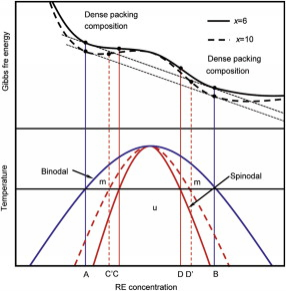
\includegraphics[width=6cm]{Diagrammi di fase/binodal.png}
    \caption{Caption}
    \label{binodal}
\end{figure}
In genere ad una data temperatura potremmo avere una fase molto più stabile dell'altra oppure una situazione in cui si hanno due minimi come in Fig \ref{binodal}. In questo caso per concentrazioni comprese tra i due punti di flesso (detti \textbf{\textit{punti spinodali}}) è favorita la decomposizione a dare due fasi distinte, mentre se la concentrazione si trova tra il punto \textbf{\textit{binodale}} (quello individuato dalla tangente alla curva) e quello spinodale si ha una fase metastabile in quanto la separazione in due fasi non è favorita (per convincersi di questi differenti trend è sufficiente ricordare la definizione di funzione concava/convessa).

\subsection{Leghe binarie}

\epigraph{[...] le temperatura di transizione (dette \textbf{\textit{incongruenti}}) non risultano un valore preciso ma un intervallo di temperatura}{\textit{Leonardo Sabattini}, I edizione}

Perchè si formino delle soluzioni completamente miscibili dobbiamo avere il soddisfacimento delle regole di Hume-Rothery cioè atomi con dimensioni simili stessa valenza ed elettronegatività e stessa struttura cristallina. In questo caso è possibile ottenere delle miscele con solubilità completa in tutto l'intervallo di composizione. Un esempio è riportato in Fig \ref{diagramma_tot_misc}.
\begin{figure}[h]
    \centering
    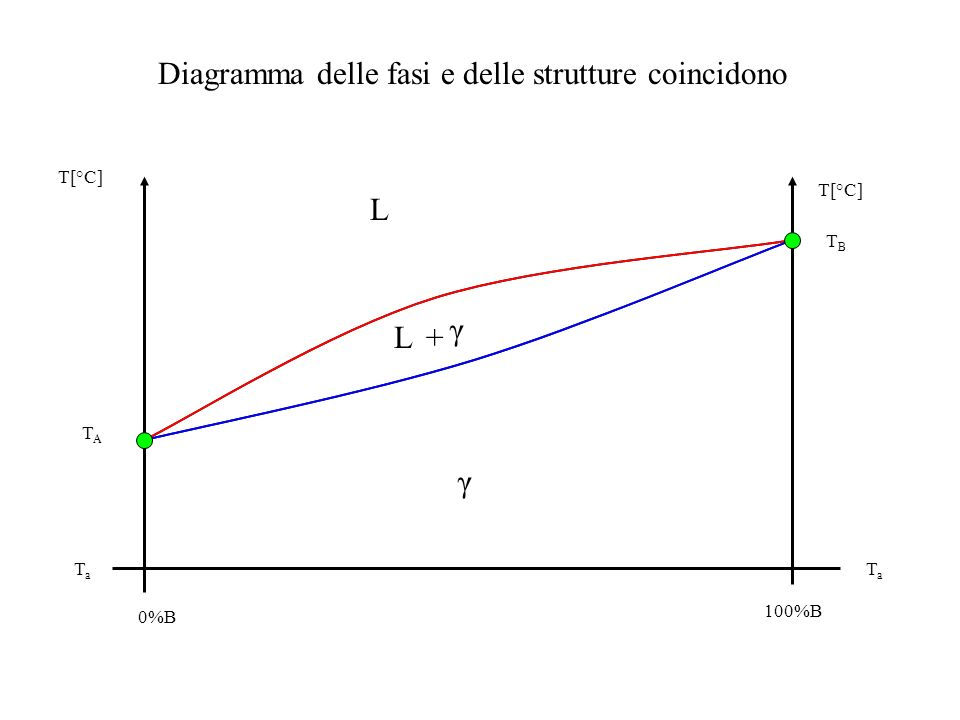
\includegraphics[width=8cm]{Diagrammi di fase/diagramma_stato1.jpg}
    \caption{Diagramma di stato di un sistema binario totalmente miscibile.}
    \label{diagramma_tot_misc}
\end{figure}

Un aspetto interessante delle soluzioni sia solide che liquide è che in generale la temperatura di transizione non assume un valore preciso, ma il processo avviene in un intervallo di temperatura. In generale, diminuendo la temperatura si arriverà nella zona intermedia in cui sono presenti sia la fase liquida che quella solida.
Se ci si trova in un punto all'interno di questa zona sono presenti due fasi ($L+\gamma$) in proporzione definita dalla lunghezza dei segmenti isotermi che congiungono il punto alle curve (vedasi \textit{regola della leva}). La fase liquida risulta arricchita del componente bassofondente mentre la fase solida risulta maggiormente arricchita della specie altofondente. Diminuendo ancora la temperatura tutta la fase liquida solidifica.\\
Queste curve sono ottenute sempre considerando casi in cui si ha il tempo necessario per permettere l'instaurarsi dell'equilibrio ed è lecito domandarsi cosa accade quando queste condizioni non valgono, in particolar modo in fase solida dove la diffusione ha minor peso. Il primo cristallita che si forma avrà composizione diversa dal liquido iniziale (ricco dell'altofondente), gli strati successivi saranno via via più poveri della specie altofondente poiché il raffreddamento repentino non riesce ad equilibrarsi e cambiare la sua composizione. L'ultimo guscio avrà composizione dell'altofondente minore della soluzione iniziale. Questo processo può generare fenomeni non voluti in quanto i bordi di grano risultano essere composti di fasi che fondono a T minore (essendo più ricchi nella fase bassofondente), e questo può causare problemi quando si lavora ad elevate temperature. Per ottenere nuovamente un sistema omogeneo non occorre sempre rifondere l'intero manufatto, ma è comunque necessario aumentare la temperatura.

\subsection{Insolubilità}

Nel caso di un sistema binario A-B solubili nello stato liquido ma insolubili nello stato solido si ha una legge del tipo:
\begin{equation}
    \chi_B=\frac{\Delta H_A(T_{m,A}-T_m)}{R \ T^2_{m,A}}
\end{equation}
Dove $T_{m,A}$ è la temperatura a cui inizia la solidificazione. Una legge analoga vale anche considerando $\chi_A$. Si osserva dunque che la temperatura di fusione in questo caso è sempre minore a quella della sostanza pura ed esiste un punto in cui si ha il passaggio diretto dalla fase solida A+B alla fase liquida, come mostrato in fig. \ref{eutettico}. Questa particolare composizione è detta \textit{\textbf{composizione eutettica}}; la temperatura a cui avviene la transizione, detta \textbf{\textit{temperatura eutettica}}, rappresenta la minima temperatura a cui può esistere la fase liquida.

\begin{figure}[h]
\begin{minipage}[b]{0.5\linewidth}
\centering
    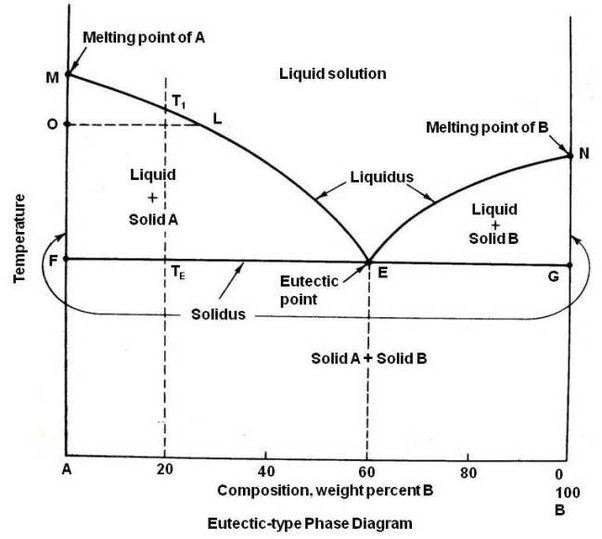
\includegraphics[width=\textwidth]{Diagrammi di fase/eutettico.jpg}
\end{minipage}

\begin{minipage}[b]{0.5\linewidth}
\centering
    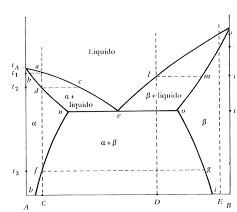
\includegraphics[width=\textwidth]{Diagrammi di fase/partial_solub.png}
\end{minipage}

\label{eutettico}
\caption{Sopra: diagramma di fase di un eutettico in una situazione di sostanze totalmente immiscibili. Sotto: diagramma di fase di un sistema a solubilità parziale.}
\end{figure}

A composizione diversa da quella eutettica si osserva una trasformazione di fase incoerente. Se ci troviamo oltre quella composizione avremo prima la formazione del cristallo B e poi la solidificazione dell'eutettico (caso \textbf{\textit{iper-eutettico}}), se invece ci troviamo prima otterremo prima la solidificazione di A e poi dell'eutettico (caso \textbf{\textit{ipoeutettico}}).
Al punto eutettico si possono osservare microstrutture di vario tipo:

\begin{itemize}
    \item \textbf{\textit{Lamellari}} o \textbf{\textit{Perliti}} in cui le microstrutture sono degli strati di fase differente.
    \item \textbf{\textit{Globulari}} dove si hanno dei cristalli sferici di una fase immersi nell'altra.
    \item \textbf{\textit{Dendritico}} dove si hanno cristalli sferici con all'interno domini lamellari.
    \item \textbf{\textit{Aciculare}} dove si hanno dei cristalli a forma di aghi immersi negli altri.
\end{itemize}

Al di fuori del punto eutettico si ha che ai bordi di grano inizia la cristallizzazione della fase a concentrazione maggiore.
Esistono altre transizioni di fase in base alle fasi iniziali e finali del processo. Queste fasi sono riportati in Fig \ref{three-phase-reactions}. Queste transizioni hanno in comune che durante la transizione la composizione non cambia e vengono detti \textbf{\textit{trasformazioni congruenti}}.
In genere a particolari valori di composizione (tali per cui si hanno rapporti interi nei numeri atomici) si possono avere dei \textbf{\textit{composti intermetallici}}, composti chimici a tutti gli effetti (ad esempio la cementite nel caso dell'acciaio).

\begin{figure}[h]
    \centering
    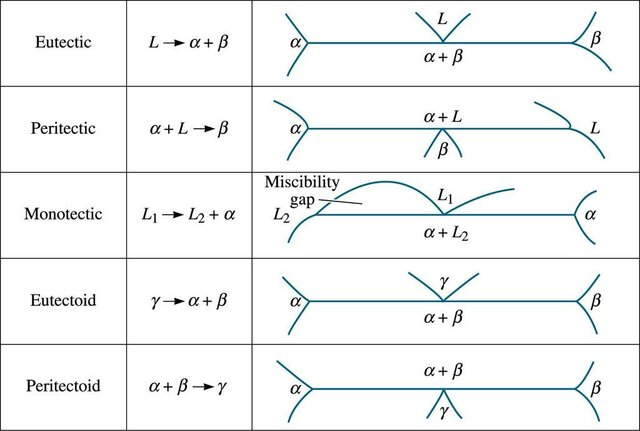
\includegraphics[width=10cm]{Diagrammi di fase/three-phase-reacctions.jpg}
    \caption{Three-phase transitions.}
    \label{three-phase-reactions}
\end{figure}

\newpage

\section{Ferro e Leghe Metalliche}

\subsection{Proprietà fisiche}

L'acciaio è una lega ferro-carbonio che presenta molte fasi differenti in base alla temperatura e composizione. La percentuale massimo di carbonio è 6,67\%. Questa percentuale non è casuale ma rappresenta la percentuale per ottenere un composto intermetallico Fe-C, la cementite Fe$_3$C. Al di fuori di questa percentuale si ha la formazione di grafite.
\begin{figure}[h]
    \centering
    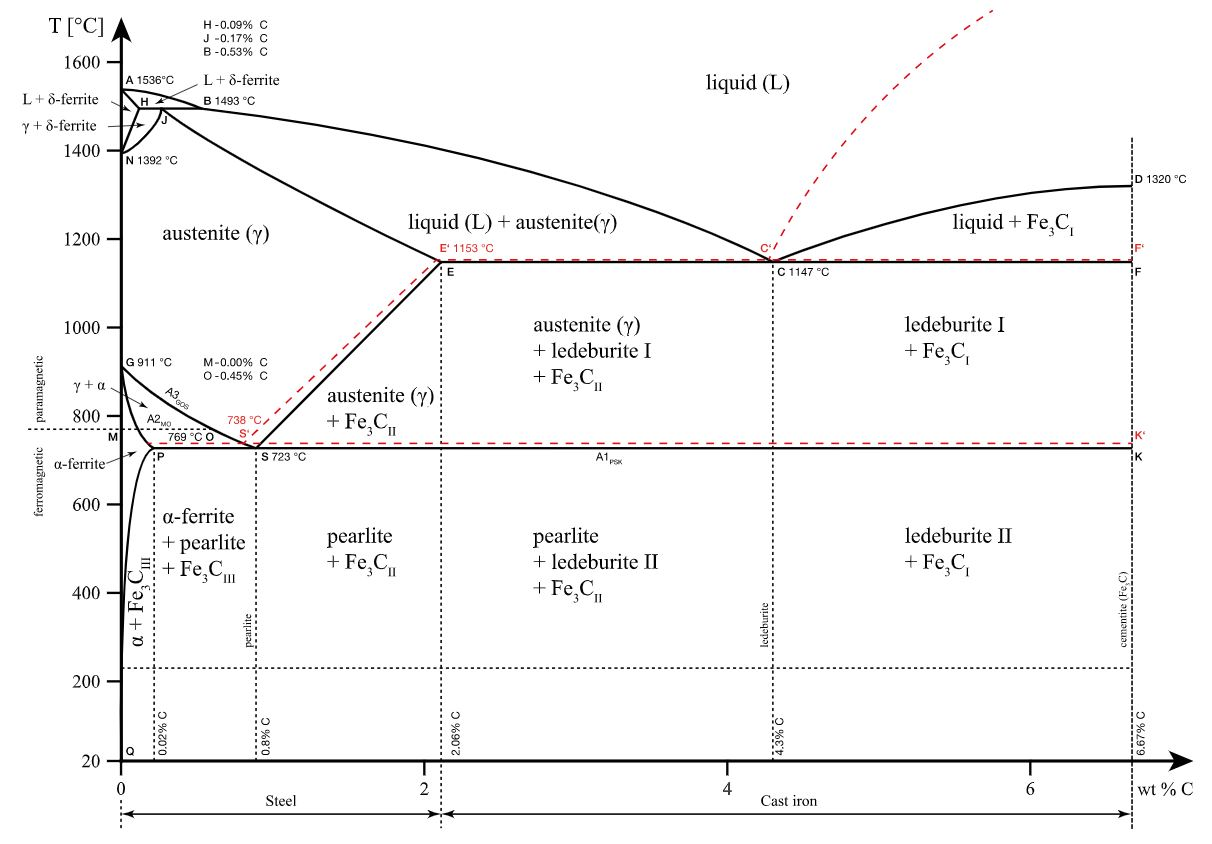
\includegraphics[width=10cm]{acciaio e transizioni di fase/Fe_phase_diagram.jpg}
    \caption{Diagramma di fase dell'acciaio.}
    \label{Steel-PhDia}
\end{figure}
Possiamo fare alcune semplici considerazioni da Fig \ref{Steel-PhDia}:
\begin{itemize}
    \item l'acciaio fonde a temperatura più elevata della ghisa (2.1\% determina il confine).
    \item l'acciaio è polimorfo e presenta più forme: Ferrite-$\delta$ (BCC), Ferrite-$\alpha$ (BCC), austenite $\gamma$ (FCC). Da notare che il passaggio da una forma cristallina all'altra comporta tensioni, in particolar modo quando la struttura cristallina è differente; inoltre è rilevante il fatto che la ferrite $\delta$ abbia un passo reticolare maggiore rispetto alla ferrite $\alpha$.
    \item La cementite $Fe_3C$ è un materiale termodinamicamente instabile ma cineticamente inerte e quindi non decompone.
    \item La solublità del carbonio nel ferro risulta incredibilmente bassa (0,02\% a 700°C), questa cosa non deve stupire in quanto il ferro è BCC e le posizioni interstiziali non sono favorevoli.      
\end{itemize}
Vediamo di capire cosa accade se raffreddiamo il nostro campione. Supponiamo di trovarci a 1000°C a concentrazione eutettoidica e raffreddiamo sotto 700 gradi, in questo caso si ottiene una struttura lamellare $\alpha$ + Fe$_3$C (perlite). La forma $\alpha$ risulta essere duttile mentre la cementite è dura e fragile ed è quest'ultima a impartire importanti proprietà di durezza agli acciai.
Se invece siamo in condizioni ipoeutettoidiche si avrà una nucleazione sui bordi di grano della componente maggioritaria (austenite), viceversa in condizioni ipereutettoidiche si avrà la nucleazione di cementite nei bordi di grano.

\subsection{Curve di Bain}

Le curve di Bain o curve TTT (time temperature transition) sono curve che descrivono le forme cristallina dell'acciaio che otteniamo a partire dalla composizione chimica e dal profilo di raffreddamento (veloce o lento).
vediamo di commentare un poco questo grafico (fig. \ref{Bain-Curves}):
\begin{itemize}
    \item La prima temperatura incontrata (720°C) è la temperatura al di sotto della quale l'austenite non è più stabile. Ogni struttura al di sotto della temperatura critica è comunque in forma $\alpha$ + Fe$_3$C.
    \item M$_s$ rappresenta la curva alla quale si ha l'inizio della transizione austenite $\rightarrow$ martensite, M$_f$ ne rappresenta la fine. Similmente sono le curve per la bainite e per la perlite. Bainite e perlite differenziano per la struttura, che è rispettivamente aciculare e lamellare.
    \item Esistono due forme differenti sia per la \textbf{\textit{perlite}} che per la \textbf{\textit{bainite}}. Se il raffreddamento è lento e diamo modo a far crescere i cristalli otteniamo la perlite grossolana, nell'altro caso otteniamo la perlite fine che presenta proprietà meccaniche superiori. La superiorità meccanica della perlite fine è dovuta alla maggior percentuale di superficie a contatto nei bordi di grano essendo la cementite e la ferrite fortemente legati tra loro. La bainite può esistere anch'essa in due forme: gli aghi possono essere paralleli al grano o ruotati di 45°. In generale le bainiti sono più lavorabili rispetto la martensite e presentano discrete proprietà a causa della cementite che rafforza la struttura.
\end{itemize}

\begin{figure}
    \centering
    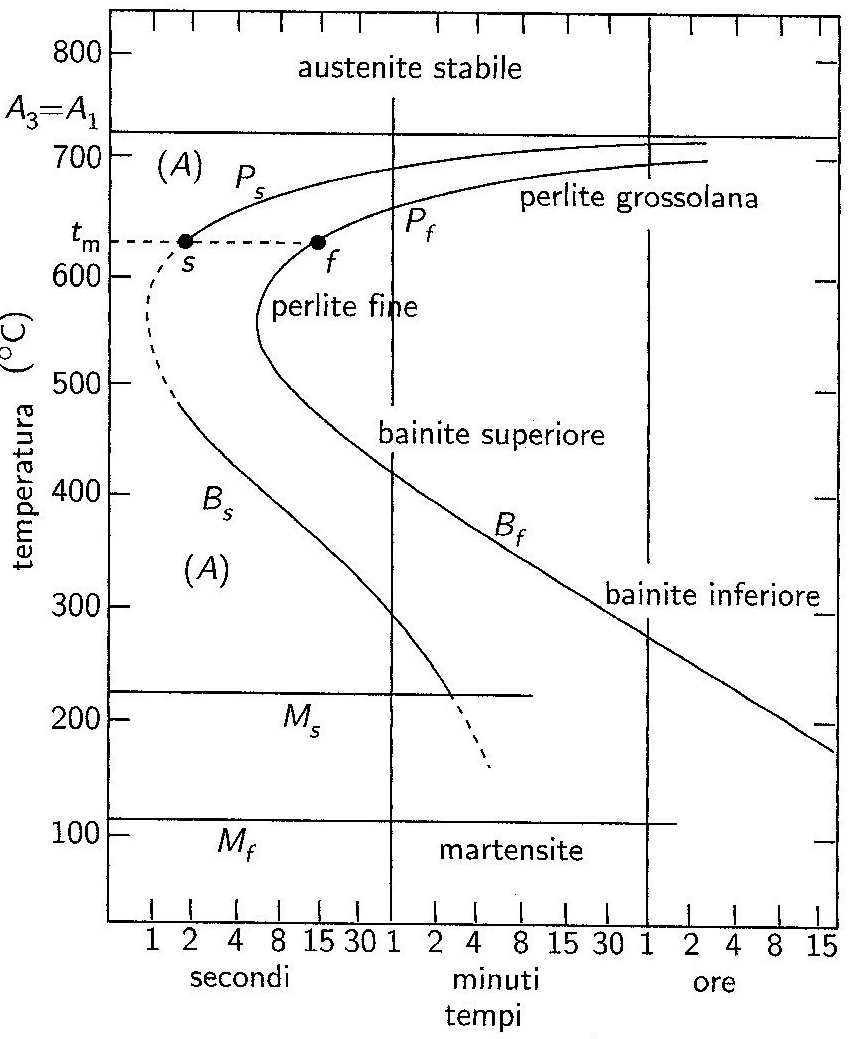
\includegraphics[height=10cm]{acciaio e transizioni di fase/Curve_bain.png}
    \caption{Curve di Bain}
    \label{Bain-Curves}
\end{figure}

La \textbf{\textit{martensite}} si ottiene per raffreddamento molto veloce, senza permettere la trasformazione da $\gamma$ a $\alpha$. Non si fornisce sufficiente tempo al metallo per riorganizzare la struttura cristallina da FCC a BCC, difatti si ottiene invece una forma intermedia (TCC, tetragonale a corpo centrato).
Questo risultato è stato ottenuto studiando i sistemi di scorrimento. 
La presenza di una maggiore quantità di carbonio aumenta l'intensità della deformazione e quindi ostacola maggiormente le dislocazioni, rendendo però il sistema più fragile.
Da notare che la possibilità di ottenere la martensite non è da ritenersi scontata, difatti se la temperatura martensitica finale (M$_f$) fosse al di sotto della temperatura ambiente non avremmo la possibilità di completare la nostra transizione ed a causa del differente volume di cella otterremo una frattura del sistema.
Per riuscire a risolvere questo problema si possono aggiungere elementi di lega, che vengono definiti:
\begin{itemize}
    \item $\gamma$-geni se aumentano l'area della zona $\gamma$ (il carbonio ad esempio, rimanendo però sotto il 2.1\%).
    \item $\alpha$-geni se aumentano l'area della ferrite.
\end{itemize}
Infatti le curve di Bain hanno una forze dipendenza dalla presenza di eventuali ulteriori specie all'interno della lega in quanto modificano il punto eutettoidico e e la temperatura eutettoidica.

\subsection{Martensite}

La martensite è ottenuta dal rapido raffreddamento della austenite (chiamata anche \textit{\textbf{tempra}}). La presenza del carbonio conferisce a questo materiale un grande punto di snervamento e grande resistenza (questi punti praticamente coincidono). Il sistema però risulta fragile e non riesce ad immagazzinare molta energia.
Esistono diversi modi di operare per aumentare il comportamento plastico dell'acciaio:
\begin{itemize}
    \item \textbf{\textit{Rinvenimento}}: Si procede al riscaldamento dell'acciaio a diverse centinaia ma comunque al di sotto della temperatura austenitica. Questo serve solamente a riattivare i moti diffusivi all'interno dell'acciaio in modo da ridurre la tensione all'interno del materiale e aumentarne la duttilità. La ripetizione di operazioni di rinvenimento e tempra è chiamata \textbf{\textit{bonifica}}.
    Da notare che il rinvenimento non elimina tutti gli effetti ottenuti dalla tempra in quanto rimaniamo sempre al di sotto della temperatura di transizione di fase. Gli acciai da bonifica vengono usati per fare gli alberi delle meccaniche e meccanismi di trasmissione a causa della loro proprietà di immagazzinare l'energia superiore a quello fresco. La forma martensitica fresca viene invece usata per fabbricare molle grazie alla loro elevata resistenza ed al loro comportamento quasi solo lineare.
    \item \textbf{\textit{Ricottura}}: in questo caso si riscalda ad una temperatura maggiore di quella austenitica e si procede ad un riscaldamento controllato. La ricottura elimina tutti gli effetti della tempra.
    \item \textbf{\textit{Distensione}}: in questo caso si procede a riscaldare il materiale ad una temperatura relativamente bassa (100-150 °C); il materiale è ancora fragile ma acquisisce una piccola porzione plastica.
\end{itemize}
Oltre a questi esistono anche altri metodi come il raffreddamento dell'austenite all'aria, detto normalizzazione (produce perliti molto fini).
\begin{figure}
    \centering
    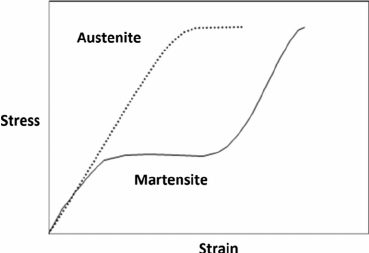
\includegraphics[width=8cm]{acciaio e transizioni di fase/Austenite-Martensite.png}
    \caption{Curva di elasticità di Austenite e Martensite}
    \label{fig:enter-label}
\end{figure}
Riattivare i processi diffusivi all'interno di un materiale ne migliora la lavorabilità e la duttilità ma ne peggiora le proprietà meccaniche. Ricordiamo però che la rigidezza non varia molto tra le varie forme dell'acciaio, dato che dipende principalmente dalle interazioni atomiche.

\subsection{Prova di temprabilità o prova Jominy}

Viene utilizzata per capire l'effetto della tempra sul materiale. Un provino fissato che si al di sopra della temperatura austenitica viene raffreddato spruzzando acqua a 24°C creando di fatto un gradiente di temperatura sulla superficie (il campione non sottoposto al raggio diretto viene raffreddato per conduzione). Successivamente viene misurata la durezza lungo l'asse.

\begin{figure}[h]
  \begin{minipage}[b]{0.5\linewidth}
    \centering
    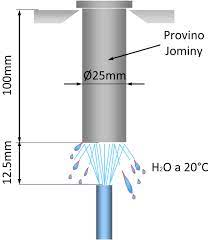
\includegraphics[width=0.6\linewidth]{acciaio e transizioni di fase/jominy test.jpg}
    \label{jominy-test}
  \end{minipage}
  \begin{minipage}[b]{0.5\linewidth}
    \centering
    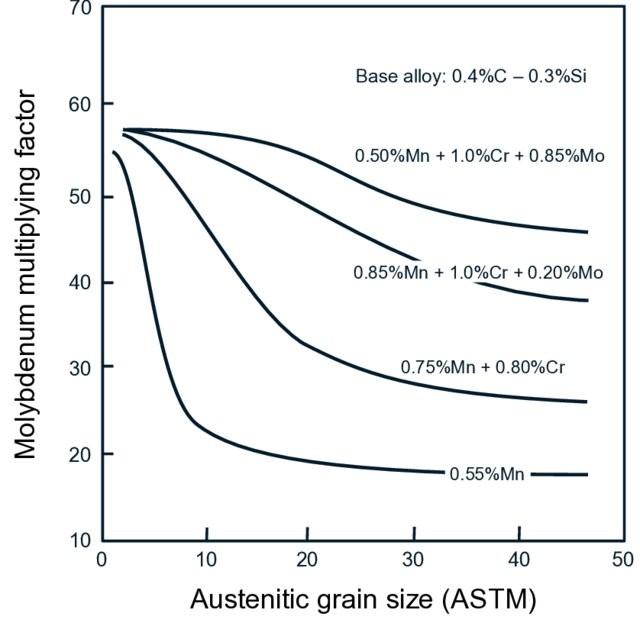
\includegraphics[width=0.7\linewidth]{acciaio e transizioni di fase/JOMINY-chart.jpg}
    \label{jominy-chart}  

  \end{minipage}
  \caption{Sinistra: setup del test. Destra: curve ottenute aggiungendo elementi di lega}
\end{figure}

All'aumentare della distanza aumenta la \% austenitica con una conseguente diminuzione della durezza. In questo test si cerca di limitare eventuali correnti convettive che trasformano le fasi austenitiche in perliti o bainiti a causa di un eccessivo raffreddamento.

\subsection{Classificazione degli acciai}

Gli acciai possono essere classificati secondo diverse categorie:
\begin{itemize}
    \item Composizione chimica (quando è nota): C\textit{X} dove \textit{X} è la $\%$ di carbonio moltiplicata per 100, o \textit{X}MgNi\textit{YZ} dove \textit{X,Y,Z} sono rispettivamente i valori percentuali moltiplicati per un fattore 100 per il carbonio e variabile per gli altri elementi di lega (si dice altamente legato se siamo sopra 5$\%$ in peso).
    \item Proprietà meccaniche (Fe250:$\sigma_R$=250 o FeE200:$\sigma_y$200). Elementi di lega come V o Cr aumentano la rigidezza del'acciaio.
    \item Gli acciai inox.
\end{itemize}

Ci sono poi gli acciai per molle: ovviamente essendo una molla vogliamo che lavori sempre in regime lineare: gli acciai martensitici freschi presentano questo tipo di comportamento; spesso si effettua una distensione per aggiungere un pezzettino plastico.
Per formare acciai duri si cerca di formare precipitati duri con opportune specie chimiche (come CW) oppure aggiungendo altro carbonio. Il trattamento viene eseguito con l'obiettivo di ottenere il picco di durezza alla temperatura di lavoro.

\subsection{Acciai inox}

Gli acciai inox sono acciai ottenuti usando il Cr come elemento di lega in proporzione maggiore del 12$\%$. Il cromo forma una patina passivante che protegge l'acciaio dalla corrosione impedendo la formazione della ruggine con conseguente rottura del materiale. Perché si formi questo strato omogeneo di cromo sulla superficie è necessario che la percentuale sia maggiore di 12 in ogni punto del materiale. La presenza di cromo comporta importanti cambiamenti al diagramma di fase dell'acciaio; bisogna comunque sempre tenere sotto controllo la quantità di cromo presente, in quanto il cromo tende a precipitare assieme al carbonio nei bordi di grano diminuendo la quantità presente nel manufatto e favorendone la degradazione.
Per evitare ciò è possibile agire:
\begin{itemize}
    \item riscaldando e sciogliendo i precipitati (non aggiusta eventuali danni ed è costoso).
    \item Usando poco carbonio (non permette però di ottenere la martensite)
    \item Utilizzando anche altri elementi di lega più affini di Cr al carbonio (ad esempio Ti).
\end{itemize}

\begin{figure}
    \centering
    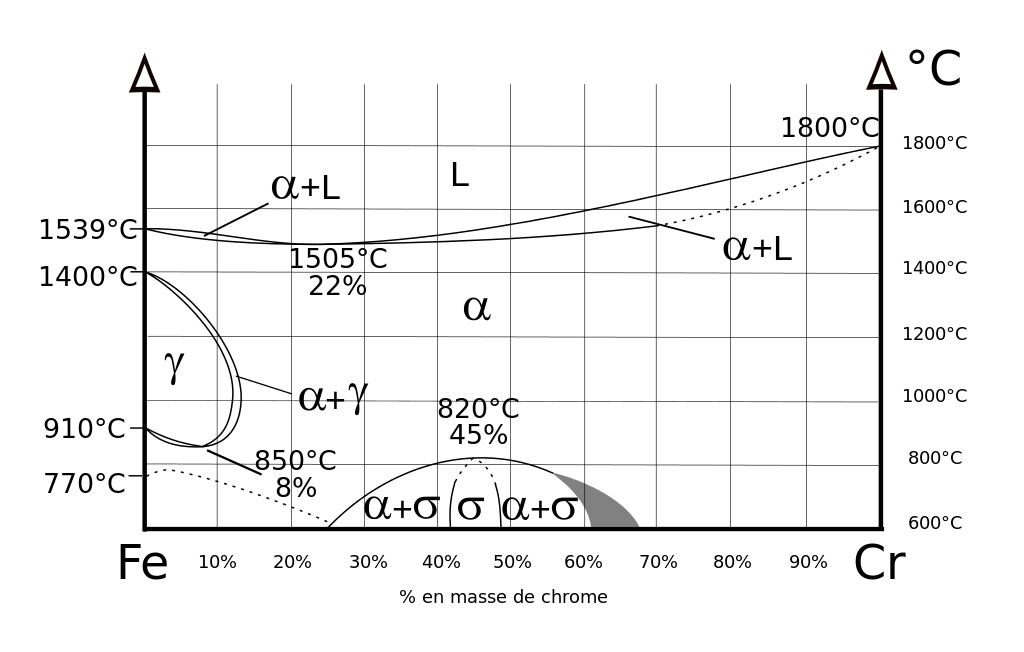
\includegraphics[width=10cm]{acciaio e transizioni di fase/Diagramme_phase_Fe.png}
    \caption{Diagramma di fase dell'acciaio inox.}
    \label{acciaio-inox.}
\end{figure}

Ci sono tre tipi di acciai inox:
\begin{itemize}
    \item Ferritici: 13\%$<$Cr$<$25\%. Sono molto dolci e poco usati a causa delle scarse proprietà meccaniche (comunque ha E=204GPa). Spesso è utilizzato come rivestimento per sistemi che non devono sopportare grandi carichi.
    \item Martensitici: non sempre sono ottenibili in quanto si ottengono per bassi tenori di cromo. Si agisce aumentando il quantitativo di carbonio che è $\gamma$-geno. Sono usati per produrre strumenti molto duri con buona resistenza alla corrosione come i bisturi o posate.
    \item Austenitici: Possono subire grandi deformazioni plastiche e contengono quantitativi di cromo importanti 18\%<Cr<25\% oltre a nichel 10\%<Ni<20\%
    \end{itemize}
Le curve di Bain in questo caso sono molto distanti e i tempi di transizione per la bainite e perlite si spostano a scale temporali molto lunghe rendendo di fatto l'austenite stabile indipendentemente dalla velocità di raffreddamento (non si vede quindi una transizione duttile-fragile). 

\subsection{Invecchiamento leghe leggere}

In leghe di Al (maggioritario) e Cu (minoritario) è possibile far precipitare il soluto (bassi contenuti, attorno al 4\%) aumentando la T.
In questo modo attraverso i moti diffusivi si genera un precipitato coerente $\theta$ che rende il materiale più resistente alle deformazioni. Aumentando troppo T si genera però un precipitato che non è più coerente $\theta"$ che rende il materiale più fragile.
In generale possiamo riassumere il processo:
\begin{itemize}
    \item Si hanno $\%$ di soluto contenute.
    \item Il processo è controllato.
    \item Si deve avere la possibilità di ottenere un precipitato coerente.
\end{itemize}

\subsection{Ghise}

Le ghise presentano una percentuale di acciaio maggiore dell'acciaio, risultando più dure ma anche più fragili (lavorano meglio con carichi statici).
Le ghise non sono saldabili e si lavorano male con macchine utensili, pertanto si lavorano per fusione. Le ghise usano per applicazioni industriali hanno un tenore che va da circa il 2.2\% al 4\%; al di sopra il tenore di carbonio è troppo elevato per utilizzi pratici.
\begin{itemize}
    \item \textbf{\textit{Ghisa grigia}}: presenta grafite in fiocchi e presenta una durezza molto elevata. Viene usata come come ammortizzatore
    \item \textbf{\textit{Ghisa globulare}} (o sferoidale): il carbonio non prende la forma di fiocchi ma di sfere. Viene principalmente usato come elemento strutturale a causa dell'elevata resistenza (350-450 MPa). 
    \item \textbf{\textit{Ghisa bianca}}: Il carbonio si trova sotto forma di cementite, sono molto fragili e si usa per ruote di carrelli o cilindri per la laminazione. Se portata a T di 800-900 °C per periodi lunghi si ha la sua solubilizzazione e si ottiene una struttura simile agli acciai da bonifica ottenendo un materiale molto più duttile.
\end{itemize}

\subsection{Lavorazione degli acciai}

L'acciaio è ottenuto a partire da vari minerali che vengono fusi nell'altoforno in cui il ferro si trova principalmente nella forma di ossido Fe$_2$O$_3$ e Fe$_3$O$_4$. Il combustibile è il carbon coke e il comburente è l'aria.  All'interno dell'altoforno la T aumenta man mano, alle temperature di lavoro si hanno le seguenti reazioni:

$$C+O_2\rightarrow CO_2$$
$$C+CO_2\rightarrow 2CO$$
$$3Fe_2O_3+CO\rightarrow 2Fe_3O_4+CO_2$$
$$Fe_3O_4+CO\rightarrow 3FeO+CO_2$$
$$FeO+CO\rightarrow Fe+CO_22$$

Ovviamente non sono le uniche reazioni che avvengono ma sono quelle che conducono alla formazione della ghisa. Oltre alla ghisa fusa si ottengono anche le scorie che galleggiano sopra la ghisa e vengono rimosse. La ghisa grezza (o grigia) appena uscita dall'altoforno trova scarsa applicazione industriale, poiché ha tenori di carbonio molto elevati e si trova sotto forma di fiocchi di grafite; tuttavia trova impiego come ammortizzatore di vibrazioni.

\newpage

\section{Frattura}

La frattura è ovviamente un evento che in ingegneria viene sempre cercato di evitare, è dunque molto importante la previsione del materiale sottoposto a sforzi per evitare che ciò accada. La modalità di frattura dipende dal tipo di materiale; esistono due tipi:
\begin{itemize}
    \item \textbf{\textit{Frattura fragile}}: la frattura fragile avviene in maniera improvvisa con la creazione di una frattura che si espande in maniera rapida senza dare nessun segno di avviso.
    \item \textbf{\textit{Frattura duttile}}: questo tipo di frattura è caratterizzata da un elevato di deformazione plastica che anticipa la rottura e che segue la crepa; inoltre è un processo più lento e stabile.
\end{itemize}

\subsection{Frattura duttile}

La frattura duttile è caratterizzata da deformazione plastica con conseguente riduzione dell'area (questo fenomeno è anche chiamato \textbf{\textit{necking}} (o strizione) ed anticipa la frattura del nostro provino. Durante lo sforzo si ha la formazione di micro-vuoti che tendono ad allargarsi ed unirsi. 
In vicinanza ai bordi, prima della rottura, la crepa inizia a seguire un angolo di 45° (che massimizza le forze di taglio); da qui viene la tipica forma "cup and cone" mostrata in figura \ref{cupcone}. Spesso questo comportamento è anche esibito da materiali in forma fibrosa.

\begin{figure}[h]
    \begin{minipage}[b]{0.45\textwidth}
    
    \centering
    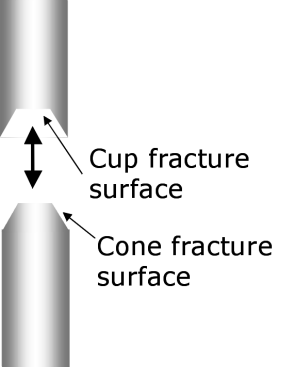
\includegraphics[height=6cm]{frattura/cup and cone.png}

    \label{cupcone}
    \end{minipage}
    \begin{minipage}[b]{0.45\textwidth}
    
    \centering
    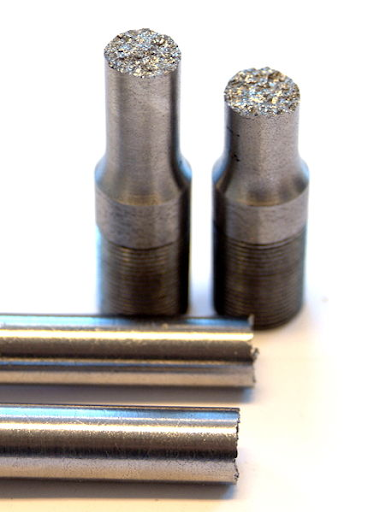
\includegraphics[height=6cm]{frattura/brittle.png}
    \label{cupcone}
    \end{minipage}
    \caption{Sinistra: frattura "cup and cone". Destra: frattura fragile.}
\end{figure}

\subsection{Frattura fragile}

La frattura fragile avviene in maniera estremamente rapida in assenza di deformazioni plastiche apprezzabili. Il piano di separazione è spesso perpendicolare alla direzione in cui è applicata la forza, con la presenza di linee che si espandono radialmente dalla crepa iniziale, spesso di forma granulare. La frattura duttile può essere di due tipi: 
\begin{itemize}
    \item \textbf{\textit{transgranulare}}: se la frattura si propaga in mezzo al grano. In questo tipo di rottura si ha la rottura dei legami atomici e la superficie appare granulosa. La frattura segue piani reticolari precisi (quelli a densità più elevata).
    \item \textbf{\textit{intergranulare}}: segue i bordi di grano. Dalla superficie è possibile vedere questi bordi di grano.
\end{itemize}
Come visto in preferenza, la frattura fragile è favorita a basse temperature.

\subsection{Test}

\epigraph{Ci sono alcuni valori che vanno considerati per la progettazione di affari}{\textit{Leonardo Sabattini}, I edizione}

La dinamica della frattura è molto complicata in quanto il fenomeno dipende da tantissimi fattori come:
\begin{itemize}
    \item Qualità della superficie.
    \item Microstruttura cristallina.
    \item Tipo di sforzo a cui è sottoposto il campione.
    \item Presenza di crepe o imperfezioni interne.
    \item Presenza di corrosione o di altre difetti dovuti all'attacco di altre sostanze chimiche.
    \item Temperatura.
    \item Design.
\end{itemize}
Esistono più metodi per studiare la frattura. La prima consiste in un provino in cui è presente un'asola di lunghezza molto minore della lunghezza del campione. Questa asola andrà a simulare la presenza di una crepa all'interno del campione. La crepa gioca in generale un ruolo molto importante nel processo di rottura, specialmente nella rottura fragile: se si osservano le linee di forza (fig. \ref{crack}) si avrà un'intensificazione di queste ultime in prossimità della frattura facendo diminuire molto lo stress richiesto per arrivare la rottura. 

\begin{figure}[h]
    \centering
    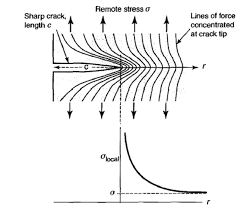
\includegraphics[width=6cm]{frattura/craks.png}
    \caption{Linee di forze in prossimità di un difetto.}
    \label{crack}
\end{figure}

Ci sono alcuni valori che vanno tenuti in considerazione per la progettazione di manufatti:

\begin{equation}
    \sigma_c=2\sigma\left(\sqrt{\frac{a}{\rho}}\right)
\end{equation}

Dove \textit{a} è la lunghezza dell'asola e $\rho$ è la curvatura dell'ellisse:

\begin{equation}
    \rho = \frac{2 a^2}{b}
    \label{eq_curvatura}
\end{equation}

Dove $b$ è l'altezza della cricca\footnote{$\rho$ rappresenta la curvatura dell'ellisse, ossia il rapporto tra il quadrato del semiasse maggiore ed il semiasse minore. Qui infatti abbiamo indicato con $a$ la lunghezza della cricca (semiasse maggiore) e con $b$ l'altezza della stessa (asse minore), da cui l'equazione \ref{eq_curvatura}}.
Il rapporto con $\sigma$ rappresenta il fattore di intensificazione.
È inoltre comune eseguire un test di trazione con un provino simile al precedente in cui è presente una cricca durante il quale si misura:

\begin{equation}
    K_I=Y\sigma\sqrt{\pi a}
\end{equation}

Dove \textit{a} è la dimensione dell'imperfezione e \textit{Y} è un parametro che dipende dal materiale. il valore di $K_I$ dipende da diversi fattori, strain rate incluso. Si va a confrontare con un valore tabulato $K_{IC}$; se $K_I$ è maggiore la frattura si propagherà, altrimenti no. Non solo crepe e difetti hanno l'effetto di aumentare localmente lo stress: anche la forma del campione è importante in quanto un design "spigoloso" agisce proprio come una crepa, un'intensificazione della forza nei punti in prossimità dello spigolo favorendo la rottura.

\subsection{Creep}

La temperatura ha un effetto molto importante sulle proprietà dei materiali. In parte questa cosa è stata discussa nel capitolo 1, in parte viene anche discussa nel capitolo sui materiali polimerici. In generale il comportamento dei materiali ad elevata temperatura (1/2 per i metalli puri, 1/3 per le leghe) è differente a cause dei moti diffusivi che sono presenti all'interno del nostro materiale ed a causa di un differente punto di snervamento. I test per lo studio del creep viene fatto a T controllata l'interno di un forno. 
\begin{figure}[h]
    \centering
    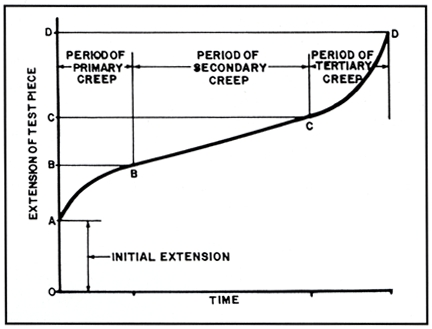
\includegraphics[width=8cm]{frattura/creep testing.jpg}
    \caption{Strain in funzione del tempo.}
    \label{creep testing}
\end{figure}
Durente il test è possibile osservare che:
\begin{itemize}
    \item Si ha un immediato aumento dello strain dovuto al comportamento elastico del materiale. Questo è seguita da una zona con una diminuzione del creep strain a causa dell'incrudimento.
    \item Si ha un seconda zona lineare in cui l'effetto dell'incrudimento e del recovery si eliminano a vicenda.
    \item Nel creep terziario la deformazione aumenta siccome ulteriori deformazioni non possono più eliminarsi tra loro.
\end{itemize}
Aumentando la temperatura o lo stress a cui è svolta la prova si osserva che la parte lineare diminuisce sempre più aumentando la sua pendenza. Diminuendo molto T e scendendo a valori molto al di sotto della T$_m$ si osserva che la parte lineare è  piatta.
Il tasso di deformazione segue una legge del tipo di Arrhenius:
\begin{equation}
    \frac{d\epsilon}{dt}=K_1\sigma^n\exp-\left(\frac{Q_e}{KT}\right)
\end{equation}

\subsection{Fatica}

Un'altra situazione che va attentamente studiata è quando il carico non è statico ma è dinamico, in quanto il pezzo potrebbe cedere anche se sottoposto a carichi molto al di sotto del punto di snervamento.
Il test consiste nel sottoporre in maniera ciclica a tensione e compressione, assieme a ciò gli si può aggiungere o meno un carico statico (cioè avere uno stress medio diverso da zero). Questa prova sarà determinata principalmente da due valori: $\sigma_m=\frac{\sigma_{max}+\sigma_{min}}{2}$ (causa strain hardening aumentano il numero di cicli necessari per la rottura) e $\sigma_r=\sigma_{max}-\sigma_{min}$.
Da questa prova si ottengono le curve di Woehler, da cui si rapporta la tensione in funzione del numero di cicli che riesce a supportare prima di cedere data una certa probabilità.

\begin{figure}[h]
    \centering
    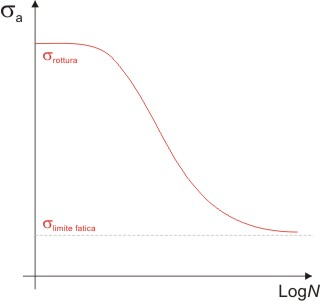
\includegraphics[width=6cm]{frattura/Curva_wohler.jpg}
    \caption{Curva di Woehler.}
    \label{Curva_wohler}
\end{figure}

Gli acciai si dimostrano ancora una volta eccezionali e spesso esibiscono un asintoto detto limite di fatica, le leghe leggere no. In generale la prova dipende da moltissimi fattori: forma del provino, stress medio e qualità delle superfici (la frattura iniziale spesso avviene alle superfici) e temperatura. Per migliorare la qualità e la durezza delle superfici si possono utilizzare varie tecniche:
\begin{itemize}
    \item \textbf{\textit{La pallinatura}}: si colpisce il campione con delle sferette molto dure in modo da provocare alla superficie dello strain hardening e quindi indurire.
    \item \textbf{\textit{Processi chimico-fisici}}: si può legare o diffondere alla superficie del nostro materiale una sostanza che diffondendosi o legandosi chimicamente alla superficie ne aumenta la durezza; un esempio sono la carburazione dell'acciaio o la nitrazione.
\end{itemize}
Anche la temperatura può provocare fatica, in quanto cambi di temperature comportano dilatazioni e contrazioni.

\subsection{Corrosione ed elettrochimica}

Un'altra fonte di difetti e di indebolimento strutturale è la corrosione ovvero l'attacco da parte di agenti chimici esterni. Data una specie ossidante (Ox) ed una riducente (Rd):
$$Ox_{ox}+Rd_{rd}\rightarrow Ox_{rd}+Rd_{ox}$$
In generale la spontaneità del processo dipende dall'equazione di Nerst:
\begin{equation}
    \Delta V=\Delta V_0+\frac{nFe}{RT}ln\frac{[Ox]}{[Rd]}
\end{equation}
Dove $n$ è il numero di elettroni scambiati e $\Delta V_0$ è il potenziale di riduzione standard; non è comunque detto che un processo spontaneo avvenga effettivamente in quanto occorre sempre considerare la cinetica. Nei processi elettrochimici sperimentalmente bisogna considerare anche i \textbf{\textit{sovrapotenziali}} ($\eta$):
\begin{equation}
    E=E_0+\eta
\end{equation}
La natura dei sovrapotenziali può essere di vario tipo, tra cui fenomeni dispendiosi energeticamente che avvengono all'interfaccia (come lo scambio di elettroni o l'adsorbimento di specie in superficie), fenomeni dovuti a gradienti di concentrazione o da una diversa mobilità degli ioni in soluzione.
Una formula del sovrapotenziale di concentrazione è data dalla relazione di Toefel:
\begin{equation}
    V=\pm\beta\ln\left(\frac{i}{i_0}\right)
\end{equation}
$\beta$ e $i_0$ sono entrambi parametri tipici della coppia redox, l'ultima è la corrente che si ha in condizioni di equilibrio quando tanta specie si riduce e tanta se ne ossida (cioè la corrente prodotta dall'ossidazione che è uguale a quella della riduzione con una corrente totale nulla, viene definita prendendone solo una delle due). In generale in condizioni stazionarie non si deve avere accumulo di carica, pertanto potenziale e corrente devono essere uguali, la condizione è dunque quando le due curve si intersecano \textcolor{red}{EH?}. Quel punto è chiamato \textit{\textbf{corrente di corrosione}} (Fig \ref{passivation}, sinistra).
Per proteggere il pezzo dalla corrosione esistono vari metodi, ad esempio:
\begin{itemize}
    \item La \textbf{\textit{passivazione}}: molti materiali metallici creano uno strato di ossido superficiale che protegge il pezzo da ulteriore degradazione modificando le curve come mostrato a destra di fig. \ref{passivation}. Non tutti gli ossidi hanno questa proprietà: nel caso del ferro si forma un ossido che si trasforma in Fe$_2$O$_3\cdot$H$_2$O, la ruggine, che ha pessime proprietà meccaniche e tende a staccarsi dal manufatto.
    \item Si può usare un anodo sacrificale, ovvero un materiale che ha un potenziale di riduzione minore del materiale che vogliamo proteggere in modo che si lui ad ossidarsi rispetto il nostro materiale.
\end{itemize}

\begin{figure}[h]
    \centering
    \begin{minipage}{0.5\textwidth}
        \centering
        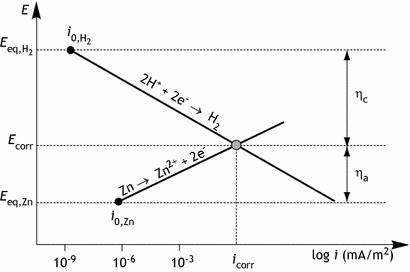
\includegraphics[width=0.7\linewidth]{frattura/tafel.png} % Sostituisci "immagine1" con il nome del tuo primo file immagine e la sua estensione
        
    \end{minipage}\hfill
    \begin{minipage}{0.5\textwidth}
        \centering
        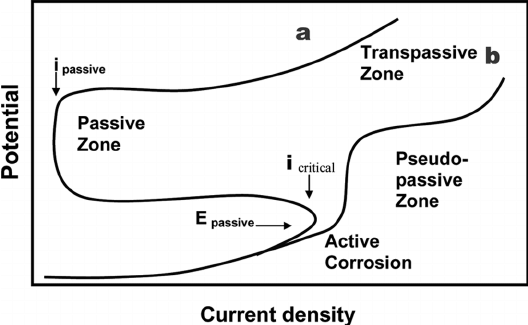
\includegraphics[width=0.7\linewidth]{frattura/passivation.png} % Sostituisci "immagine2" con il nome del tuo secondo file immagine e la sua estensione
        
    \end{minipage}
    \caption{Sinistra: relazioni di Tafel, Destra: effetto della passivazione}
    \label{passivation}
\end{figure}

La corrosione dipende da molti fattori, ad esempio temperatura, che di solito ne aumenta la velocità, presenza di umidità (l'ossidazione del ferro avviene solo in presenza di acqua), e concentrazione di protoni. La corrosione nel caso del ferro avviene per areazione differenziale: all'interno della goccia di acqua non si ha una concentrazione uniforme di ossigeno, ma cambia a seconda dalla distanza dell'interfaccia. Questo gradiente di concentrazione assieme alla presenza di protoni causa l'ossidazione del ferro nelle zone in cui la concentrazione di ossigeno è maggiore. Un'altra fonte di corrosione sono le giunzioni con metalli più nobili, dove essenzialmente il metallo nobile funge da anodo sacrificale.

\newpage

\section{Materiali ceramici}

Le ceramiche sono materiali inorganici costituiti da metalli o non-metalli. Riconosciamo essenzialmente tre tipologie di ceramiche:

\begin{itemize}
    \item \textbf{\textit{Ceramiche tradizionali}} contenenti argilla (permette la lavorazione), silice (componente refrattario) e feldspato (è una fase fine che si disperde e funge da legante).
    \item \textbf{\textit{Vetri inorganici}} basati sul silicio e raffreddati senza permette la cristallizzazione.
    \item \textbf{\textit{Ceramiche avanzate}} basata su ossidi, carburi e nitruri.
\end{itemize}

I ceramici sono materiali duri e fragili, con valori molto bassi di duttilità, bassa resistenza e tenacità; queste proprietà sono però modulate dalla classe specifica e dalla natura del legame chimico. A seconda della composizione chimica i ceramici presentano legami covalenti (nel caso di composti omopolari come grafite e diamante) che hanno un elevata direzionalità, oppure da legami ionici che non presentano una vera direzionalità \textcolor{red}{EH?}. La maggior parte dei composti ionici presenta anche un certo carattere covalente in funzione dell'elettronegatività.

I materiali ceramici essendo molto vari tra di loro trovano impiego in vari campi. In generale presentano una densità maggiore dell'acqua ma minore dei metalli (2-4 g/cm$^3$), sono resistenti in compressione con un modulo dell'ordine di 1000 MPa (5000 per il diamante) ma sono deboli in trazione con un valore dai 5 ai 10 volte minore (vedi tab. \ref{tab:ceramic_properties}); questo è sopratutto causato da difetti ed imperfezioni alla superficie ed all'interno del cristallo (ad esempio dei vuoti nel campione) che limitano le proprietà meccaniche di questi materiali. Il modulo di Young e la T$_m$ dipendono molto dalla struttura cristallina; il più delle volte T$_m$ non permette di lavorare questi materiali per fusione e vengono usati come materiali refrattari, inoltre hanno anche un basso coefficiente di espansione termica. Inoltre presentano valori di durezza incredibilmente elevati permettendo il loro impiego come abrasivi. Di seguito sono riportati alcuni valori di proprietà meccaniche di qualche materiale ceramico:

\begin{table}[h]
\centering
\begin{tabular}{lccc}
\hline
\textbf{Material}     & \textbf{Traction (MPa)} & \textbf{Compression (MPa)} & \textbf{Elastic Modulus (GPa)} \\ \hline
Allumina               & 200 - 400                          & 2000 - 4000                          & 300 - 400                       \\ \hline
Zirconia              & 200 - 1000                         & 1000 - 2000                          & 200 - 400                       \\ \hline
Silicon Carbide       & 300 - 600                          & 2000 - 4000                          & 400 - 500                       \\ \hline
Silicon Nitride       & 500 - 1000                         & 2000 - 5000                          & 200 - 320                       \\ \hline
Boron Nitride         & 100 - 300                          & 100 - 500                            & 100 - 400                       \\ \hline
\end{tabular}
\caption{Traction, compression strength and elastic modulus of ceramic materials}
\label{tab:ceramic_properties}
\end{table}

Le ceramiche sono caratterizzate da un comportamento fragile che dipende molto dalla presenza di difetti interni e di superficie, trovano dunque impiego strutturale se usati se devono resistere a carichi di compressione. La dipendenza da difetti interni è direttamente collegata al processo di produzione ed anche alla natura stessa del composto, dunque ogni campione presenta delle differenze strutturali interne (che possono essere particolarmente importanti tra due campioni diversi) e pertanto i vari test di trazione non danno un valore preciso ma piuttosto un range. Per migliorare la capacità in trazione difatti si operano processi per creare stati di compressione.
Il metodo di produzione determina anche la porosità del materiale; spesso i ceramici vengono prodotti a partire da polveri. La porosità nel materiale ha un effetto deleterio sulle proprietà meccaniche del nostro materiale (sia sulla rigidezza che sulla resistenza). Si può arrivare a perdere anche il 50\% in resistenza a causa di una porosità del 10\%:
\begin{equation}
    \sigma_{fs}=\sigma_0\exp(-nP)
\end{equation}
Dove $\sigma_{fs}$ è la resistenza alla flessione ed $n$ una costante sperimentale. Altro elemento da tenere in conto è la dimensione del campione: dimensioni maggiori implicano possibilità maggiori di avere cricche all'intero del materiale.

\subsection{Struttura dei ceramici}

La struttura dei cristalli dipende principalmente dal rapporto dei raggi delle specie presenti nel reticolo cristallino. In generale gli anioni sono più grandi dei cationi e questi ultimi andranno ad occupare le posizioni interstiziali del cristallo. 
Se il rapporto tende ad 1 si avrà numero di coordinazione 8 ed il catione si troverà al centro del cubo come nel caso del CsCl. Nel caso di ZnS (zincoblenda) invece lo zinco occupa i siti tetraedrici (la metà per rispettare le corrette proporzioni) all'interno di una cella FCC di zolfo. Il più facile è NaCl con una coordinazione ottaedrica. In generale esistono tanti sali e quindi tante possibili forme diverse. Altre strutture più esotiche ma comunque importanti ed abbondanti sono le perovskiti e gli spinelli.
I materiali ceramici non sono necessariamente cristalli ma possono essere anche solidi amorfi, come il vetro, in cui la silice non ha un pattern periodico ma è disposto in maniera casuale; occorre specificare che la silice presenta anche forme cristalline (Fig \ref{silice}) di vario tipo con la struttura che si organizza con tetraedri di SiO$_4^{4-}$ e può formare anche pattern piuttosto complicati.

\begin{figure}[h]
    \centering
    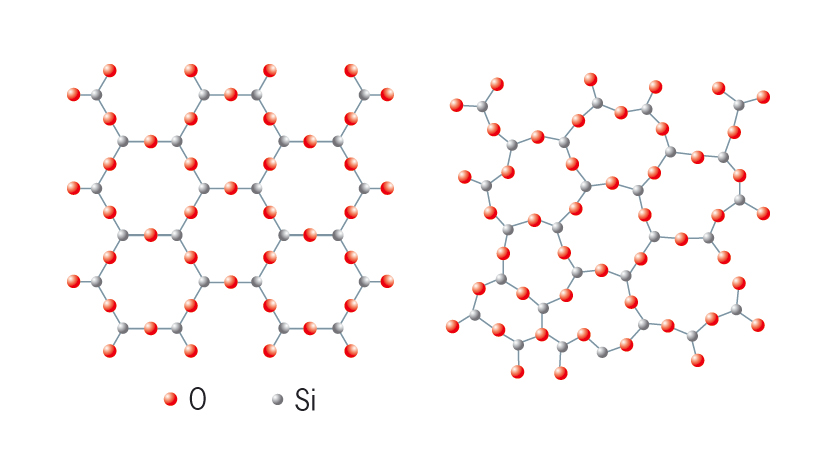
\includegraphics[width=8cm]{ceramici/silice.jpg}
    \caption{Silice amorfa e silice cristallina}
    \label{silice}
\end{figure}

I ceramici cristallini inoltre non presentano dislocazioni: infatti in un solido ionico lo scorrimento degli atomi è quasi impedito, dato che porterebbe alla rottura quasi certa per i composti ionici (lo scorrimento di due filari di atomi porterebbe ioni di segno opposto vicini tra loro, favorendo la rottura del campione); per i covalenti è invece possibile, ma si ha comunque elevata direzionalità. Nel caso di solidi amorfi, non avendo una struttura regolare, non si parla di dislocazione ma piuttosto di processi di tipo viscoso.

\subsection{Ceramiche avanzate}

I ceramici avanzati sono molto duri e spesso vengono impiegati nella produzione di utensili inoltre spesso presentano una tenacità maggiore rispetto ad altri materiali ceramici
\begin{itemize}
    \item Allumina: è utilizzato nei sistemi in cui occorre operare ad alta T mantenendo elevata resistenza meccanica, Trova impiego anche in molti alti campi a causa delle sue proprietà isolanti, abrasive e refrattarie.
    \item Zirconia: è utilizzata come materiale refrattario o aggiunto in altri materiali ceramici. Ha applicazioni simili all'allumina. Presenta diverse transizioni di fase aumentando la T: da tetragonale$\rightarrow$monoclina(1200)$\rightarrow$cubica(2400) fino a fusione (2700). Si può ottenere una forma di zirconia tenacizzata stabilizzando la forma cristallina cubica aggiungendo ossidi al reticolo.
    \item SiC: principalmente usato a causa del suo alto T$_m$ e delle sue sue resistenze a ossidazione ad alta T (maggiori del T di fusione dell'acciaio). è usato come ricopertura nei compositi di Carbonio-Carbonio, è usato anche come abrasivo o come refrattario. L'applicazione più interessante è sicuramente quella da semiconduttore anche ad alta temperatura.
    \item Si$_3$N$_4$ proprietà simili al SiC ma le sua resistenza all'ossidazione alte temperature è leggermente minore. Si prepara insufflando N$_2$ direttamente su Si
    \item Diamante: è usato, oltre che in gioielleria, come abrasivo o come rivestimento per altri materiali.
    \item Silice (SiO$_2$): è l'ingrediente principale del vetro, è possibile creare abrasivi, usarlo come refrattario o come isolante. Può essere anche usato per creare fibre.
    \item TiO$_2$: spesso è usato come pigmento bianco per le superfici o come rivestimento per le medicine. Viene impiegato anche nella protezione di raggi UV.
\end{itemize}

\subsection{Lavorazione}

\begin{itemize}
    \item Sintesi (CVD, decomposizione termica  metodi in soluzione) o estrazione.
    \item Macinazione e mescolamento in acqua o a secco. 
\end{itemize}
Si usano diversi metodi per la sintesi, molti dei quali richiedono l'uso della pressione:
\begin{itemize}
    \item Pressatura a secco: viene usato per materiali ad uso refrattario e per componentistica per elettronica (è unidirezionale).
    \item Pressatura isostatica: Il processo HIP consiste nel porre un oggetto in un ambiente gassoso ad elevata temperatura e elevata pressione isostatica. Lo stampo in questo caso è ermetico e flessibile (di solito di natura elastomerica). Si può lavorare sia a secco che in presenza di un mezzo come acqua o altri tipi di lubrificanti. Viene usato per produrre mattoni, materiali refrattari ed altri tipi di ceramiche.
    \item Hot pressing: le tecniche viste in precedenza con l'uso anche di temperature elevate che permetto di rendere i nostri materiali molto rigidi e ad elevata densità.
\end{itemize}

\begin{figure}[h]
  \begin{minipage}[b]{0.5\linewidth}
    \centering
    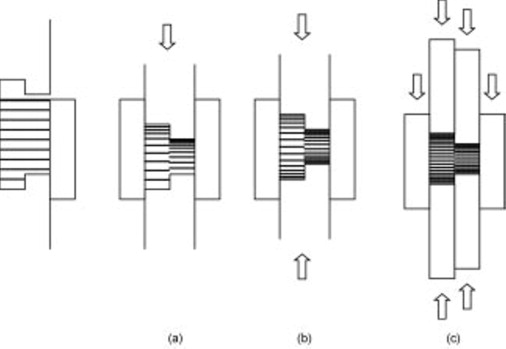
\includegraphics[width=\linewidth]{pressing.jpg}
    \label{pres}
  \end{minipage}
  \begin{minipage}[b]{0.5\linewidth}
    \centering
    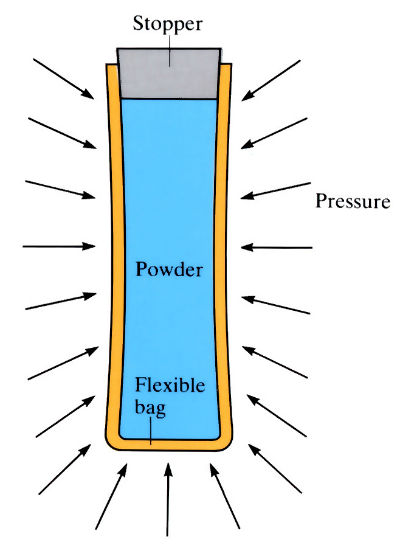
\includegraphics[width=\linewidth]{iso_pressing.jpg}
    \label{iso-pres}  

  \end{minipage}
  \caption{Sinistra: pressatura. Destra, pressatura isostatica}
\end{figure}

Se il materiale lo permetto è anche possibile procedere per fusione a scorrimento (slip casting). Si cola il liquido in un contenitore che assorbe il liquido in cui è contenuto il nostro materiale ceramico. Il materiale in eccesso viene rimosso ed il nostro pezzo viene asciugato e cotto. Anche l'estrusione è un metodo.
I materiali ceramici possono essere sottoposti a diversi trattamenti termici:
\begin{itemize}
    \item Drying or binders removal (si rimuove l'acqua o il solvente organico).
    \item sinterizzazione: pressione+temperatura per avviare processi diffusivi e generare così nuovi oggetti. Una maggiore T di sinterizzazione produce ceramiche con porosità minori
    \item vetrificazione: formazione di una fase vetrosa.
\end{itemize}
Cose sulle fratture e sul fatto che le ceramiche presentano sempre microfratture ed altre cose che ne peggiorano le proprietà. Il fatto che i cristalli possono subire def plastiche solo su particolari piani di scorrimento, in solidi policristallini questa cosa è pressoché impossibile. Pericolosità di fratture superficiali da cui possono espandersi altre cose.
Vetri: silice amorfa e cristallina: vari tipi di additivi: ossidi dei metalli alcalini e ossidi che si integrano nel network: allumina, ossido di titanio e di piombo.
Vari tipi di vetro. Viscosità nei vetri. e produzione vetri. NaCL è FCC ma non è una struttura compatta: gli ioni sulla diagonale non si toccano. CN 12 significa che le dimensioni dell'anione e catione sono uguali. Spinelli, 
Metodi di rafforzamento meccanico e chimico.

\subsection{Ceramici tradizionali}

I materiali ceramici tradizionali sono ottenuti mescolando argilla, silicati e feldspati in varie proporzioni. Il legante è l'acqua che dà luogo ad una serie di reazioni chimiche che modificano le proprietà del materiale. Un vantaggio di questa classe di materiali sono plasticità e malleabilità che permettono al campione di essere lavorato facilmente (\textbf{\textit{idroplasticità}}). La lavorazione può procedere anche per slip casting: una sospensione di argilla o di altro materiale è versata all'interno di uno stampo con le superfici porose in modo tale da avere la deposizione della sospensione. Una volta rimosso il liquido rimane uno strato che per essiccamento diventa solido. In generale questi ceramici richiedono l'essiccamento per rimuovere l'acqua in eccesso, e questo può essere ottenuto lasciando il materiale all'aria oppure riscaldandolo con calore o con IR. Altre volte invece si si può procedere anche alla cottura del pezzo per ottenere proprietà meccaniche differenti. Il materiale a base di argilla ad alte temperature può iniziare a fondersi e creando uno strato di liquido esterno che va a tappare tutte le porosità presenti \textbf{\textit{vitrificazione}}.

\subsection{Vetri}

I vetri sono un'importante categoria di ceramici. Sono principalmente composti da silice amorfa a cui vengono aggiunti vari ossidi (di metalli alcalini o di altri elementi) per modificarne le proprietà chimico-fisiche e renderli adatti a particolari impieghi:
\begin{itemize}
    \item La presenza moderata di B$_2$O$_3$ aumenta la sua resistenza chimica e trova impiego come vetro di laboratorio.
    \item Se in presenza maggiore conferisce al vetro resistenza alle elevate temperature ed allo shock termico e si ottiene il vetro chiamato Pyrex.
    \item Il vetro più impiegato è quello che contiene ossidi di calcio, sodio e magnesio; il principale motivo per cui vengono aggiunti questi ossidi è quello di modificare la composizione chimica del vetro e ridurne la temperatura di fusione.
    \item Vetri ricchi ($>$10\%) di B$_2$O$_3$, Al$_2$O$_3$ e CaO si ottengono dei vetri che possono essere trasformati in fibre (le fibre di vetro appunto).
\end{itemize}
Il grado di cristallizzazione del vetro dipende molto dal rate di raffreddamento e possiede curve simili a quelle di Bain in cui si possono avere fasi vetro-ceramiche se il campione è portato ad opportune temperature; in ogni caso il vetro amorfo è un liquido "super raffreddato" (il grafico del suo volume specifico non presenta una discontinuità a T$_m$ ma un cambio di pendenza a T$_g$).\\
Il vetro può essere rinforzato con la tempra che consiste nel riscaldamento di quest'ultimo rimanendo al di sotto della temperatura alla quale il vetro non riesce più a mantenere la propria struttura senza apparenti deformazioni. I
Il raffreddamento è eseguito lasciando il pezzo caldo all'aria; le superfici del vetro si raffredderanno più velocemente dell'interno mentre l'interno ancora plastico tenderà a contrarsi di più di quanto l'esterno glielo permette (il raffreddamento è seguito da una contrazione, se il raffreddamento è molto veloce la contrazione è minore) creando uno stato di compressione che aumenta la resistenza alla frattura. La forza necessaria a creare la frattura all'esterno deve essere in grado di favorire questa compressione residua. Un altro tipo di tempra è la tempra chimica in cui gli ioni di sodio all'interno del vetro vengono scambiati con del potassio aumentando la resistenza all'impatto, al graffio e alla flessione.
Le ceramiche vetrose trovano largo impiego come materiale dielettrico e per la loro compatibilità biologica.\\
La lavorazione del vetro dipende molto dalla sua viscosità e quindi dalla sua temperatura:
\begin{equation}
    \eta=\eta_0\exp\left(\frac{Q}{RT}\right)
\end{equation}
A temperatura molto elevata la sua viscosità e bassa a sufficienza da permettere la lavorazione. Il raffreddamento può essere critico in quanto lo shock termico può causare la rottura di quest'ultimo.
Un metodo per ottenere un raffreddamento più controllato è l'uso di stagno fuso: alla temperatura di fusione dello stagno il vetro è già solido. La modellazione del vetro invece avviene spesso per stampaggio e per soffiaggio.
%%%%%%%%%%%%%%%%%%%%%%%%%%%%%%%%%%%%%%%%%%%%%%%%%%%%%%%%%%%%%%%%%%%%%%%%%%%%%%%%%%%%%%%%%%%%%%%%%%%%%%%%%%%%%%%%%%%%%%%%%%%%%%%%%%%%%%%%%%

\newpage

\section{Compositi}

\epigraph{Infine è particelle di SiC o Allumina diametro di qualche micron per aumentare la rigidezza del metallo}{\textit{Leonardo Sabattini}, I edizione}

I materiali compositi sono formati da due o più materiali differenti. Un composito è di solito costituito da: 
\begin{itemize}
    \item un \textbf{\textit{filler}} (o \textit{riempitivo}) che ha la funzione di rinforzo, è aggiungo come fibra o come particelle. È il componente che andrà  sostenere gli sforzi meccanici.
    \item  una \textit{\textbf{matrix}} (o \textit{matrice}) che ricopre completamente il filler, ha il compito di unire e trasferire lo stress all'altra fase.
\end{itemize}
La forza dei materiali compositi è la capacità di presentare proprietà intermedie tra i due materiali che lo costituiscono ma complessivamente superiori. Le proprietà finali dipendono da molti fattori: il rapporto matrice/filler, la struttura del filler (fibre continue o discontinue, particellare) ed anche i metodi di lavorazione (spesso questa classe di materiale è fortemente anisotropa). 
La classificazione dei compositi dipende dal tipo di matrice usata:
\begin{itemize}
\item \textbf{\textit{Polymeric matrix composites (PMC)}}. Ne esistono diversi tipi, un esempio sono le fibre di vetro ottenute a partire dalle resine insature di poliestere e le fibre di carbonio o kevlar resine epossidiche. Le proprietà di questa classe di compositi possono avere direzionalità specifiche in quanto spesso composto da fibre. Ovviamente anche il metodo di produzione influisce: è possibile limitare l'anisotropia facendo in modo che l'orientazione delle fibre sia multidirezionale (ad esempio tramite stacking di piani di fibre orientate ad angoli diversi). Le fibre di vetro sono prodotte da particolari tipi di vetro con alto contenuto di ossido di alluminio (15\%); in base a come sono intrecciate si ha una differente resistenza. Le fibre di carbonio sono ottenute dal PAN (poliacrilonitrile). Dopo un trattamento a 200-400°C per ossidare le fibre di PAN si ha una pirolisi a 400-600°C in atmosfera inerte o a 600-1500°C per avere delle fibre grafitiche. La grafitizzazione che si ottiene a 1800°C aumenta il grado di orientamento dei cristalliti (?). L'ultima classe di PMC molto importanti sono le fibre aramidiche che trovano impiego sopratutto per la produzione di oggetti protettivi sia dalle alte temperature sia dagli urti (antiproiettili ad esempio). Hanno una basse densità, si deconpongono a T elevata e hanno una buona resilienza e forza meccanica. Sono fatte a partire da poliammidi aromatiche. 
 
\begin{table}[h]
\centering
\begin{tabular}{@{}lcc@{}}
\toprule
\textbf{Materiale}  & \textbf{Resistenza ($MPa$)} & \textbf{Modulo di Young ($GPa$)}  \\ \midrule
Poliestere & 40 - 90  & 55 - 130  \\
Resina epossidica & 55 - 130 & 2.8 - 4.2 \\
Fibra di vetro-poliestere (intrecciata) & 206 - 344 & 103 - 310 \\
Fibra di carbonio (unidirezionale)-Resina Epossidica & 1860 (65 a 90°) & 145 (9.4 a 90°) \\ \bottomrule
\end{tabular}
\caption{Proprietà meccaniche di alcuni PMC}
\label{tab:resine}
\end{table}

\item \textbf{\textit{Metallic matrix composites (MMC)}}. Anche di questa classe ne esistono di vario tipo: fibre continue, fibre discontinue o particellari. Le fibre continue come fibre di ossido di alluminio, grafite, tungsteno, boro o SiC si ottengono pressando queste lamine a caldo direttamente sul metallo e servono per aumentarne la rigidità e resistenza meccanica. Questa cosa è sopratutto usata per le fibre leggere nel settore aerospaziale. Un altro tipo sono le fibre discontinue come i "whiskers" di SiC (diametro di qualche micron e lunghezza di diverse decine); queste si ottengono per hot pressing, aggiunta di polveri ed estrusione o infiltrazione nei metalli fusi, anche qui si osserva un aumento della resistenza meccanica e della rigidezza. Infine è possibile utilizzare particelle di SiC o allumina diametro di qualche micron per aumentare la rigidezza del metallo. In fibre di alluminio continue si arrivano a valori di Tensile Strength di 1500 MPa e modulo elastico di 220 GPa ma un allungamento massimo di 0.810\&, le fibre discontinue e particolare arrivano a circa 500 MPa e 120 GPa con allungamenti di pochi punti percentuali mentre i materiali privi di rinforzo hanno Tensile strength inferiore a 500 MPa e modulo elastico inferiore ai 100 GPa ma un allungamento del 10\%.

\item Ceramic matrix composites (CMC). Anche nelle fibre ceramiche si aggiunge fibre continue di SiC (\textcolor{red}{chiedere come sono le fibre continue di SiC} o ossido di alluminio o paricelle e Whiskers di SiC con un conseguente aumento della resistenza meccanica e resistenze alle frattura. Vengono aggiunte per CVD o hot pressing. Servono sopratutto a modificare ed arginare la propagazione delle crepe all'interno del materiale e formare dei ponti tra le crepe.
\end{itemize}

\subsection{Comportamento meccanico}

Il tipico comportamento meccanico dei compositi inizia con un comportamento elastico sia da parte del filler che della matrice: questi tendono ad allungarsi fino a quando uno dei due (di solito la matrice) entra in regime plastico e quindi si osserva un cambio di pendenza nel grafico stress-strain. Una volta raggiunto l'allungamento massimo del filler il composito inizia a cedere senza avere un cedimento della struttura netto e catastrofico in quanto il filler è ancora nel regime plastico. Inoltre un altro vantaggio è che le crepe non si propagano in tutto il filler ma sono limitate dalla matrice. \textcolor{red}{RISISTEMARE CHE LEO L'HA SCRITTA ALLA CAZZO DI CANE}

In generale la risposta meccanica del materiale dipende dalla composizione del materiale anche perché le forze esterne sono trasmesse dalla matrice al filler attraverso le forze di taglio. Per materiali binari avremo:
\begin{equation}
    E_c=E_fV_f+E_mV_m
\end{equation}
Dove V$_m$ e V$_f$ sono le frazioni in  e $E_c$ è il modulo di Young del composito.
Esistono due regimi in cui può lavorare un composito: il primo è il regime di \textbf{\textit{isostrain}} (Fig \ref{isostress-isostrain}  sinistra) in cui  entrambi i materiali sono sottoposti allo stesso allungamento, un questo caso si ha che $\epsilon_f=\epsilon_m=\epsilon_{c}$ ed inoltre si ha $P_f+P_m=P_c$, il carico sarà dunque distribuito secondo la seguente formula.
\begin{equation}
    \frac{P_f}{P_m}=\frac{\sigma_fA_f}{\sigma_mA_m}=\frac{\epsilon_fE_fA_f}{\epsilon_mE_mA_m}=\frac{E_fA_f}{E_mA_m}
\end{equation}
Nelle condizioni di \textbf{\textit{isostress}} (Fig \ref{isostress-isostrain} destra) invece la direzione della forza è ortogonale al piano della fibra si hanno condizioni diverse: $\sigma_c=\sigma_f=\sigma_m$; $\Delta l_c=\Delta l_f+\Delta l_m$. In questo caso si ha:
\begin{equation}
    \frac{1}{E_C}=\frac{V_f}{E_f}+\frac{V_m}{E_m}
\end{equation}
\begin{figure}[h]
    \centering
    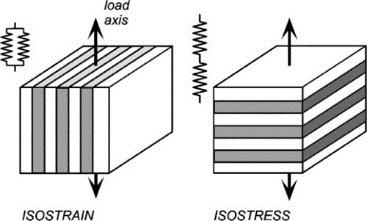
\includegraphics[width=8cm]{isostress-isostrain.png}
    \caption{Condizione di isostress ed isostrain.}
    \label{isostress-isostrain}
\end{figure}

La frattura nei compositi è un processo complesso in quanto spesso si ha una matrice duttile e un filler fragile e resistente. In genere durante la deformazione il materiale duttile si comprime e gli eventuali vuoti tra le interfacce dei due materiali scompaiono. Quando lo stress si trasmette dalla matrice al filler ed il filler inizia a deformarsi, il materiale non riesce più a deformarsi efficacemente e la fibra inizia a rompersi in maniera fragile. Se il legame è debole si possono creare dei vuoti tra le fibre e la matrice (cavitazione). Infine se lo stress è applicato in maniera ortogonale alle lamine si può avere delaminazione comportando la rottura del materiale.
Nel caso del calcestruzzo o di altri compositi formati da particelle grosse disperse il meccanismo è diverso in quanto il rafforzamento è dato dall'ostruzione della matrice; per particelle fini invece queste agiscono sul movimento delle dislocazioni impedendolo, come accade nel caso del precipitation hardening anche se con effetti minori.
Nel caso di fibre, il suo comportamento dipende dalla direzione e dalla lunghezza di queste, quando la lunghezza è corta e l'orientazione è randomica l'efficienza è minore e le proprietà peggiori. Le fibre possono anche trovarsi sotto forma di whiskers (cristalli praticamente perfetti) e mostrano i valori massimi di resistenza ottenibile essendo quasi del tutto privo di difetti.

\subsection{Metodi di lavorazione}

\epigraph{i nostri materiali messi a panino vengono compressati a T e P elevata unire il filler e la matrice.}{\textit{Leonardo Sabattini}, I edizione}

Molti manufatti compositi sono ottenuti per stampaggio seguito da essiccamento all'aria (\textbf{\textit{open molding}}).
\begin{itemize}
    \item \textbf{\textit{Hand lay-up}}: il materiale viene colato in uno stampo aperto. Le resine o fibre aderiscono alla superficie prendendo la forma dello stampo.
    \item \textbf{\textit{Spray lay-up}}: il materiale viene colato in uno stampo aperto depositato attraverso uno spray; questa tecnica è preferita quando si vogliono avere fibre sottili. Eventuale aria residua viene eliminata con rulli o attraverso processi simili, anche qui segue essiccamento a temperatura ambiente o superiore.
    \item \textbf{\textit{Vacuum Bag-Autoclave}}: viene principalmente usato per fare lamine dalle elevate proprietà tecnologiche. Le resine già cariche di filler \textcolor{red}{chiedere a milazzo}. Dovrebbe consistere in fogli di resina carichi di fibre che una volta in autoclave a T elevata comporta l'unione dei due pezzi.
    \item  \textbf{\textit{Filament winding}}: consiste nell'intrecciare fili di fibra saturi di resina in modo da ricoprire una superifice i quali induriranno quando esposti all'aria.
\end{itemize}
Un'altra classe di lavorazioni la si ha quando si lavora al chiuso (\textbf{\textit{closed molding}}):
\begin{itemize}
    \item \textbf{\textit{Compression molding and transfer molding}}: i due componenti messi a panino vengono pressati assieme a T e P elevata per unirli in maniera permanente.
    \item \textbf{\textit{Resin transfer molding}}: è simile al precedente ma se prima si pressavano assieme lamine diverse ora si inietta all'interno dello stampo la resina liquida che andrà a legare al filler.
    \item \textbf{\textit{Sheet-molding compound (SMC)}}: in questo processo lamine differenti vengono pressate attraverso rulli e riscaldate.
    \item \textbf{\textit{Reinforced Reaction Injection Molding (RRIM)}}: in questo processo due o più resine vengono scaldate separatamente e poi unite a fibre di vetro macinate. La miscela viene iniettata in uno stampo ad alta pressione e le si lascia prendere la forma dello stampo.
    \item \textbf{\textit{Pultrusione}}: viene utilizzata per produrre manufatti in forma allungata come barre o filamenti. Prevede di far passare un filamento continuo di filler in un bagno di resina per saturarlo e successivamente attraverso acciaio riscaldato.
\end{itemize}

\newpage

\section{Cemento}

Il cemento è un ceramico, il calcestruzzo e il cemento armato invece sono compositi. Il cemento è fatto da una polvere contenente silicati di calcio e alluminati:
3CaOSiO$_2$ silicato tricalcico, 2CaOSiO$_2$ silicato bicalcico, 3CaOAl$_2$O$_3$, 4CaOAl$_2$O$_3$Fe$_2$O$_3$. Alla polvere viene aggiunta acqua per creare la malta (che spesso non presenta proprietà adeguate ma comunque si può usare per elementi che non sono sottoposti a particolare carichi).
Aggiungendo degli aggregati di grana grossa, come bricciolino o pietre, e di grana fine, come la sabbia, si ottiene il calcestruzzo. L'acqua aggiunta funge da legante trasformando i silicati in silicati idrati e idrossidi:
$$2C_3S+6H_2O\rightarrow C_3S_2\cdot3H_2O+3Ca(OH)_2$$ 
Il cemento è un legante idraulico e ha bisogno di subire un processo di solidificazione durante la quale si essicca. Dopo la solidificazione abbiamo il calcestruzzo. La cinetica di solidificazione dipende dalla scelta di composizione (\textbf{\textit{mix design}})) la quale viene scelta in base alla classe di resistenza, alla classe di esposizione, dimensione degli aggregati ed al rapporto acqua/cemento, che deve essere superiore a 0.2 (di solito è compreso tra 0.4 e 0.5). Poca acqua porta a legami incompleti e maggiore fragilità, troppa acqua a porosità troppo elevata.
Esistono 5 tipi di cemento \textcolor{red}{QUANDO L'HA FATTO?}
\begin{itemize}
    \item Cemento ordinario
    \item Cemento resistente ai solfati
    \item Cemento presa rapida, il calcestruzzo normalmente è pronto dopo 28 gg; ovviamente l'essiccamento rapido si ripercuote sulle proprietà del materiale e risulta più soggetto a fessurazioni.
    \item Cemento a basso calore di idratazione, che viene usato per le grandi opere per evitrare la fessurazione
    \item Cemento molto resistente ai solfati
\end{itemize}
I solfati sono chimicamente pericolosi per il cemento; inoltre il cemento non ha proprietà meccaniche eccezionali, essendo un ceramico, il calcestruzzo invece cede all'interfaccia con il filler. Di solito sul cemento, oltre ai soliti test di compressione e tensione, vengono effettuati altre prove: uno per controllare il rapporto acqua-cemento, il test a 45° e la prova di flessione. Il modulo elastico del cemento è calcolato a partire dalla classe di resistenza: $R_{ck}$:
\begin{equation}
    E_c=5700\sqrt{R_{ck}}
\end{equation}

\subsection{Calcestruzzo armato}

Il calcestruzzo armato è ottenuto rinforzando il calcestruzzo con barre d'acciaio per compensare la scarsa resistenza a tensione. La loro quantità dipende dal carico previsto:
\begin{itemize}
    \item Presentano spesso una forma elicoidale per aumentare la superficie e dunque la presa.
    \item Lo spazio tra interfaccia e le colonne di ferro è detta copriferro ed è molto importante in quanto evita l'ossidazione dell'acciaio e dunque il cedimento del pezzo.
    \item I rinforzi sono fatti di comune acciaio da costruzione, in ogni caso la prima cosa a cedere è l'interfaccia. 
\end{itemize}
Una cosa che si deve considerare è a presenza di eventi sismici in quanto sottopone il materiale a flessione.
Esistono due metodi per preparare il calcestruzzo:
\begin{itemize}
    \item Calcestruzzo armato precompresso: viene preparato in casseforme dove sono presenti delle barre d'acciaio d'acciaio tirate. Quanto il cemento viene rimosso dalla cassaforma l'acciaio tende a ritirarsi creando uno strato di compressione nel calcestruzzo aumentandone la resistenza in flessione (i ceramici non hanno buone resistenza in trazione).
    \item post-teso: il pezzo viene preparato colando il calcestruzzo in una cassaforma dove sono presenti le barre d'acciaio ricoperte da guaine e lasciate solidificare. Una volta pronto vengono tirate le barre d'acciaio lasciando uno stato di tensione e introducendo la malta nelle guaine 
\end{itemize}

\newpage
\section{Materiali Polimerici}
I polimeri sono materiali formati da molecole a catena molto lunga in cui si ha la ripetizione di un'unità più piccola detta \textbf{\textit{monomero}}. Esistono vari tipi di polimeri in base alle loro proprietà, una possibile classificazione è:
\begin{itemize}
    \item \textbf{\textit{Termoplastici}}: i materiali termoplastici possono essere fusi e diventano più duttili all'aumentare della temperatura; sono gli unici che possono presentare un certo grado di cristallinità.
    \item \textbf{\textit{Termoindurenti}}: Non possono essere fusi poichè comporta la rottura dei legami e si ha un aumento del modulo elastico all'aumentare della temperatura; sono sempre amorfi. 
    \item \textbf{\textit{Elastomeri}}: permettono di allungarsi di diverse volte il loro valore iniziale (anche x10); sono sempre amorfi.
\end{itemize}
Le proprietà di un polimero vanno ricercate direttamente nella loro composizione.
In generale ci possono essere più monomeri diversi: omopolimero se il tipo di monomero è solo 1, copolimero random se sono disposti casualmente, alternato o a blocchi o graft (con il back-bone di un tipo e le ramificazioni di un altro). Il tipo di polimero dipende molto dal metodo in cui è stato prodotto. I polimeri statistici, random e alternati di solito hanno proprietà intermedie ai singoli omopolimeri. Questa cosa permette di modulare le proprietà in base alla composizione.
Il polimero a blocchi o ramificato mostra proprietà tipiche di ogni monomero inoltre questi possono mostrare nuove proprietà a causa del legame chimico tra le catene non uguali. la presenza di \textbf{\textit{cross-links}} è estremamente importante ed incide fortemente le proprietà del polimero. Perchè si formino \textbf{\textit{cross-links}} è necessario la presenza di gruppi funzionali che permettano la creazione di nuovi legami. Un'altra cosa che determina fortemente le proprietà del polimero è il peso molecolare. In generale sperato un certo valore di soglia non si ha una sostanziale differenza nelle proprietà anche se si ha un aumento molto grande della viscosità ed un conseguente aumento nella difficoltà di lavorazione. Eisstono più modi di calolare la massa dei polimeri, è possibile fare una semplice media aritmetica o mmedie pesate. Il rapporto tra la media pesata e la media aritmedica si chiama \textbf{\textit{polidispesione o heterogenity index (PDI)}} e ci dice quanto è omogenea la composizione all'interno del nostro polimero. \textcolor{green}{immagine viscosità vs peso molecolare e proprietà}. Il \textbf{\textit{grado di polimerizzazione}} è calcolato come il numero di unità presenti calcolati a partire dalla massa media. Nel caso di copolimeri la massa usata è una media pesata sulle frazioni molari. Alla'mentare della massa si osserva un'aumeto della durezza e si passa da cere o solidi malleabili a solidi duri. I polimeri possono presentare un certo grado di cristallinità in base a diversi fattori. 
\subsection{Termoplastici}
La proprietà principale dei termoplastci è la possibilità di poter essere rimodellati diverse volte. Non tutti i materiali possono essere cristallizzati ed a più si ottengono strutture semi-cristalline. Le fasi cristallina posseggono un $T_m$ al di sopra della quale la fase cristallina diventa liquida; quelli amorfi invece possseggono la gass transition temperature in cui da un solido vetroso (duro) si ottiene uno stato rubbery (duttile). Le T$_m$ sono relativamente basse a causa della debolezza dei legami intercatena; T$_m$ e T$_g$ aumentano all'aumentare della rigidezza e delle forze intermolecolari.
\textcolor{green}{tabella}
\subsection{Elastomeri e termoindurenti}
La caratteristica principale di queste due classi è la presenza di cros-links, i primi hanno una bassa densità di cross-links, la seconda molto elevata. L'elasticità di questi materiali si basa su  entropy recovery mechanism. La csa da tenere in considerazioe è che una volta formati i cross-links questi materiali non possono essere ulteriormente lavorati.
\subsection{polimerizzazione}
\begin{itemize}
    \item chain growth
    \item step growth
\end{itemize}
Possono procedere per addizione o condensazione: il polietilene si ottiene per polimerizzazione radicalica a catena (è un addizionr), questo itpo di tecnica viene usata per monomeri insaturi. In questo tipo di polimerizzazione la catena che sta crescendo ha una reattività maggiore del singolo monomero (difatti è un radicale) ma indipendente dalla dimensione della catena stessa. Alti livelli di polimerizzazione sono ottenuti anche a basse coneversioni in quanto la crecita è indipendente, l'aumento del rate di conversione spesso si riflette sul numero di polimeri ottenuti più che sul grado di polimerizzazione in quanto una volta che la catena è morta non reagisce èiù.
Illustriamo ora gli step di crscita:
\begin{itemize}
    \item Inizializzazione ad opera di luce/calore/radicale. La polimerizzazione inizia a causa della presenza di radicali, una specie molto reattiva che da luogo ad una reazione a catena. La formazione del radicale può avvenire attraverso da degli iniziatori che formano radicali se sottoposti a radiazione o a calore.
    \item Propagazione: il radicale si "trasferisce" quando il monomero si lega alla catena. Nel caso del cloruro di vinile (per fare il PVC) si hanno due possibilità di propagazione (testa-testa o testa coda), la probabilità rispetta diversi fattori come l'energia di attivazione dei due processi e la stabilità termodinamica dei due radicali; nel caso del PVC la forma più stabile è quella che presenta il radicale nel cabronio legato al cloro. 
    \item terminazione : può avvenire per diversi motivi: due catene che si stanno propagando si combinano, si può avere disproporzione tra le due catene o si può avere trasferimento di catena.
    \end{itemize}
\subsection{carrelata di polimeri}
    \begin{itemize}
        \item PE: bassa densià, bassa resistenza ma alto strain (600\%). tre tipi: HDPE, LLDPE, LDPE. Viene usato per imballaggi e rivestimenti e come isolante elettrico. pf 110
        \item PVC: amprfp, fragile, alta resistenza chimica, rogodo ma poco resiliente, difficilemnte lavorabile. Può essere unito con diversi additivi: lubrificanti per migliorare la lavorabilità, fillers per abbatterne i costi, pigmenti per colorarlo. stabilizzanti termici (composti organimetallici). Usato er giubbotti waterproof, tetti delle macchine, film e containers.
        \item Poliproilene pbasso costo, buona durezza superficiale e discreta resistenza all'midità, calore e agli agenti chimici. è usato per fare container, oggetti domesitici, 
        \item Polistirene fragile e non flessibile e trasparente. La resistenza può essere aumentato con l'aggiunta di polibutadiene. Facilmente processabile ed a basso costo. Scarsa reistenza agli agenti atmosferiche. è usato anche per gli imballaggi sottoforma di polistirolo.
        \item PAN (poliacrilonitrile) fibra per vestiti, buona resistenza maeccanica e stabilista chimica
        \item SAN poslistirebe e acrilonitrile.  EIgido duro e trasparente. Pannelli e lentied anche tazze o cose per uso domenstico o vetri di sicurezza.
        \item PTFE 
        \item Polimetilacrilato (PMMA): plexiglass 
        \item ABS (acrilonitrile/butadiene/polistirene): buona resistenza meccanica e resistenza chimica, le proprietà cambiano in base alla composizione
    \end{itemize}
    \subsection{step-growth polimerization}
    Richiede che il monomero abbia almeno due gruppi funzionali.
    La crescita non è spontanea e la reazione avviene lentamente e monomeri e polimeri presentano reattività pressoche invariata. Il grado di polimerizzazione continua a crescere all'aumentare della conversione. Possono coinvolgere due specie diverse  una specie dello stesso tipo. avviene per reazioni successive. Le reazioni sono spesso policondensazioni. Un esempio è il PET che è fatto a partire da acido ftalico e glicole etilenico. I poiesteri sono fatti a partire da biacidi e alcoli, le poliammidi (nylon) a partire da ammine e acidi carbossilici. Policarbonati, polisulfoni. Se invece abbiamo la formazione di un legame tra monomeri senza prodotti scondari si parla di poliaddizione linear come nel caso delle resine epossidiche. L network step policondansation consiste in due step:
    formazione di prepolimeri a bassa massa e successivo raggiungimento di alti livelli di crosslinks dopo aver sottoposto il campione a calore. Tipici monomeri sono l'urea ed il fenolo o la formaldeide. Alcuni esemoio sono le resine fenoliche. La anche l'addizione può formare networs come il caso del DGEBA che da luogo a strutture ramificate a partire da epossidi e diammine. gelazione: all'aumentare della conversine si ha un aumento non lineare della viscosità, Superato un certo punto (quando le dimensioni delle molecole sono comparabili con quelle del sistema) il nostro materiale non si comporta più come un liquido e diventa immobilizzato, le molecole possono ancora muoversi ma attraversp la diffusione; questo impedisce la conversione completa. Due modi di prevedere Carothers e flory. Il primo sovrastime $p_c=\frac{
    2
    }{f_{av}}$ assume che la gelazione avviene a lunghezza infinita, cosa falsa; il secondo sottostima ($p_ap_b)_c=\frac{1}{f-1}$non tiene in conto effetti intramolecolare che possono creare loop e spostare a conversioni più alte il punto di gelazione.
    \subsection{Cristallinità nei polimeri}
    Alcuni polimeri possono cristallizzare raggiungendo un certo grado di cristallinità (mao completa). Il graod massimo dipende da tanti fattori:
    \begin{itemize}
        \item La velocità di raffreddamento, la tatticità, la massa molare, la presenza di additivi come agenti nucleanti o la presenza di catene laterali. La crisytallizzazione può essere evitata raffreddando molto velocemente il polimero, la cristallizzazione può essere indotta dopo con l'annealing ad una temperatura tra $T_g$ e $T_m$. Livelli pi alti di cristallizzazione possono essere ottenuti se si raffreddano i polimeri a partire da soluzioni diluite piuttosto che dal fuso a causa di assenza di fattori sterici. La struttura tipica è la lammellae. Esistono diversi difetti (immagine). La presenza di gruppi polari da direzionalità al tutto, siu ha un legame selettivo tra particolari gruppi funzionali.  meccanismo adjacent e random re-entry (come si formano le lamelle. Sferuliti: sono simili ai grani dei metalli.
        Condizioni da soddisfare per la cristallizazione
    \end{itemize}
    temperatura di fsuione: non è un valore preciso ma un range, dipende dalla storia del campione, dipende dal rate di riscaldamento. Inoltre dipende dalla struttura chimica, dalla massa molare, dalle ramificazioni e dalla copolimerizzazione. Come trovare la glass transition a partire dal volume specifico. i tipi di polimeri che danno $T_g$ e i vari statii (mettere immagine di slide 87. vedere slide 90, molto importante, praticamente dice che i materiali cross linked dopo la T$_g$ presentano un moldulo di Young crescente al crescere della temperatura. Caoutchouc: polisopropilenne (mettere la formula) c'è sia il cis edd il trans, quest'ultimo tende a cristallizzare invece. L'aggiunta di zolfo e il riscaldamento genera la gomma, quella vulcanizzata è molto più resistente. GOmme sintetiche: polistrirene+polibutadiene (SBR per le gomme) , oliacrilonitrile+butadiene per appicazioni in cui è richiesta maggior resistenza chimica e meccanica. Policloropìprene (1-clorobutadiene o neoprene) buona resistenza chimica e meccanica, è usato per ricoprimenti e cavi. Gomma di silicone (struttura) Isolante.
    \subsection{Proprietà meccaniche}
    For some polymers, strong stretching with a stress 
minimum and break at a much higher stress is 
observed. 
This phenomenon is known as strain hardening and stress induced crystallization. It is caused 
by orientation and alignment of polymer chains parallel to the load which increases both 
strength and stiffness of the plastic in stretch direction.
Comporatemento degli elastomeri: allungamento pazzesco a bassi strain ed improvviso aumento dello stress prima della rottura, occhio sempre a strain rate, T densità di cross links, peso molecolare, composizione e microstruttura (esempio di polimero con microstrutture molto diverse).
Effetto di T sulla rottura, si osserva una transizione brittle to fragile (spesso coincide con T$_g$) a volte è minore come il PC. Comportamento viscoelastico: materiali entanglati leggermente (come gli elastomeri) daranno grandi deformazioni elastiche  prima di rompersi, quelle non crosslinkate come i termoplastici daranno.
\textcolor{red}{il comportamento elastico non è necessariamente lineare? perhce all'aumenatre di T i termoindiìurenti induriscono? dopo il T glass i termoindurenti rammolliscono? infine anche gli elastomeri si comportano così?}compostamento viscoelastico. Il comportamento viscoelastico si osserva al di sopra di T$_G$. Nel regime viscoelastico si ha una dipendenza dal rate e dal tempo in cui è stato sottoposto il carico. I materiali viscoelastici sono materiali che in parte hanno un comportamento elastico (legge di hooke) ed in parte tipico dei materiali liquidi (legge di Newton), la natura della risposta del polimero cambi al variare di T, a bassa t il regime elastico domina, ad alta T l'incontrario.
legge di newton:
\begin{equation}
    \tau=\eta\frac{d \epsilon}{dt}
\end{equation}
Esistono diversi modelli tutti fatti da molle e pozzetti. Creep function (??). Ogni modello ha i suoi vantaggi e svantaggi (vedere Lazzeri). Boltzmann superposition principle :  linera viscoelasticity ha come assunzione questo principioo.  La somma delle deformazioni è la somma algebrica dello strain a causa dei step di carico. ALla fine è possibile scrivere le cose come somma (che si approssima ad intergale che si traduce in una convoluzione quando si fa la trasformata.
In generale la trasformata del modulo elastico è complesso:
\begin{equation}
    E(\omega)=E'(\omega)+E"(\omega)
\end{equation}
La parte complessa è associata all'energia dissipata per ciclo mentre la parte reale è l'energia immagazzinaa, il rapporto di parte reale e parte complessa e definita come \textbf{\textit{damping factor}}:
\begin{equation}
    \tan(\delta(\omega))=\frac{E'(\omega)}{E"(\omega)}
\end{equation}
In generale è possibile plottare E in funzione della frequenza, i picchi possono essere considerati come effetti di damping ad una frequenza caratteristica di transizione o rilassamento del processo associato al particolare moto dei polimeri.
\textcolor{green}{aggiungere i grafici} Dai grafici si vede che se la frequenza del carico è lenta si ottiene lo stesso effetto di alzare la temperatura. Vicevera ad alta T si comporta come un solido vetroso.
gnificant damping occurs at Tg when the applied test frequency matches the 
natural frequency for main-chain rotation. At higher frequencies, there will be 
insufficient time for chain uncoiling to occur and the material will be relatively 
stiff. On the other hand, at lower frequencies, the chains will have more time 
to move and the polymer will appear to be soft and rubbery. n general, in any viscoelastic system, the transition process associated to a 
particular type of molecular motion can be observed not only by a change in 
the timing of the stimuli, but also by a change in the diffusivity of the system, 
i.e. by a change in the temperature at which the response is tested. \textcolor{green}{mettere grafici dei presenti in slide 115}. It is thought that there is a general equivalence between time and temperature. 
For instance, a polymer that displays rubbery characteristics under a given set 
of testing conditions can be induced to show glassy behaviour by either 
reducing the temperature or increasing the testing rate or frequency. 
In generale due curve calcolate a T' e T e a frequenze differenti $\omega$ e $\omega'$ mostrano la sressa compilance ma a T differenti, esiste solamente un shift factor $\alpha$ che dipende esclusivamente da T. la funzione di $\alpha_T$ è fittata con la WLF euation che ha due parametri diversi in base ai vari polimeri. In uno spettro di G in funzione della temperatura (o della frequenza)si possono osservare diversi picchi, questi picchi sono dovuti a diverse transizioni dette primarie e secondarie. Ogni transizione è associata ad un particolare moto molecolare.queste analisi si effettuano con il DMTA dynamic mechanical thermal analysis. Mettere un paio di immagini spiegando bene la compilance e cosa c'è in ogni grafico.  The average molecular mass of chains primarily affects the mechanical resistance since 
a minimal degree of polymerization is mandatory in order to obtain a mechanically 
stable solid with appreciable stiffness and resistance. However, beyond a critical level 
of molecular mass there is no more increment of both mechanical stiffness and 
resistance with the length of the chain.
 As the crystallinity degree grows, for a fixed quantity of material, both tensile strength, 
elastic modulus and density are increased. Anche la struttura del cristallo è importante per la determinare le proprietà meccaniche. La presenza di gruppi laterali aumenta il modulo di Young poichè impedisce il movimento delle catene polimeriche. Anche la presenza di gruppi molto polari aumentano molto la resistenza meccanica. Anche gruppi laterali molto ingombranti stericamente. L'uso di fibre di vetro comportanoun un aumento delle proprietà della resistenza meccanica. é possibile definire il modulo di creep ($mc=\sigma/\epsilon(t)$ e lo stress relaxation (stessa cosa ma ciò che varia nel tempo è il carico.
\subsection{Frattura nei polimeri}
può essere duttile o fragile o una cosa intermedia. a T inferiore della T$_G$la frattuura è per lo più di tipo fragile, viceversa duttile. La frattura fragile è spesso accompagnata dalla formazione di zone cave e di fibre in cui i polimeri sono altamente allineati. (quesdte zone sono chiamate craze.la formazione del craze e diversa da quella di una frattura in quanto la craze può ancora supportare carico finchè nonsi arrriva ad una elongazione tale da rrivare alla rottura.La frattura duttile avviene quando è possibile lo slipping e quindi la deformazione plastica del materiale. nel processo anche qui si formano delle fibre a causa della forza.
\subsection{Ciclo industriale}
Si parte dai materiali raw (petrolio) per poi ottenere i monomeri. Si fa la polimerizzazione o direttamente su stampi o si ottengono prima pellets, polveri o soluzioni liquide che comunque richiederanno ulteriori processi. ci sonodiversi modi per poliaddizione:
\begin{itemize}
    \item in \textbf{bulk}: qui la concentrazione di monomero è massima ed il processo relativamente  più semplice dando alti rates di polimerizzazione e bune conversioni, inoltre è spesso difficiel rimuovere efficacemente il calore (anche a causa dell'elevata viscosità) dal sistema e la viscossità aumenta moto rapidamente. Si usa poco inizializzatore per ridurre il rate e si usano basse conversioni al costo di recuperare il monomero non reagito.
    \item In soluzione sia il monomero che il polimero che l'inizializzatore sono sciolti. Il solvente deve ridurre complessivamente la viscosità  e permettere ko scambio di calore. La concentrazione di monomero e minore inoltre bisogna rimuovere il solvente (per evaprazione) o riuscendo a far precipitare il polimero. filtrazioni e centrifugazioni fanno il resto.
    \item in sospensione serve per evitare probei causati dl trasferimento di calore ma con a reazione che si comporta come fosse nel bulk. IL medium deve essere inerte nei confronti delle altre specie involte. Spesso si usa l'acqua limitando la temperatura di lavoro a 70-90 gradi. 
    \item in emulsione. Qui The reaction components differ from those used in 
suspension polymerization only in that the initiator 
must not be soluble in monomer but soluble only in the aqueous dispersion medium; questa cosa modifiva il meccanismo e la cinetica di polimerizzazione e anche il prodottocreando un particolato di polimero in acqua conosciuto come Latex.
    \end{itemize}
    Only for thermosets:
    \begin{itemize}
        \item estrusione
        \item injection moluding (valido anche per i ternoindurenti, la cura si fa nello stampo.)
        \item bubble film blowing
        \item Thermoforming
        \item blow moulding
        \item compression moulding
    \end{itemize}
La frattura all'interno dei polimeri dipende molto dal grado di cristallinità. 

\section{Viscoelasticità-Lazzeri}
Ora andremo a descrivere un poco meglio le proprietà di un materiale polimerico.
Come accennato in precendenza, i polimeri sono una classe di materiali che permettono estensioni molto grandi in cui non si può più ragionare in termini di allungramento puramente elastico. La \textbf{rubber-like elasticity} è caratterizzata curve stress-strain in cui si arrivano a valori di strain fino a 10x il valore iniziale, caratterizzato da non linearità estesa. Per ottenere queste proprietà è necessario un certo grado di cross-linking, in caso opposto la le catene polimeriche scorrono l'una sulle altre creando così delle deformazioni non elastiche.
Come accennato in precedenza, queste proprietà dei polimeri sono dovute principalmente a motivi entropici più che a motivi termodinamici, in quanto l'ordine aumenta quando il materiale e sottoposto ad una forza esterna.
Ci sono diversi modelli che spiegano questa iper-elasticità:
\begin{itemize}
    \item Modello della freely jointed chain: considera il polimero non come una struttura da angoli definiti in cui son presenti atomi ma come un insieme di elementi rigidi di lunghezza fissata e assume che tutte le configurazioni abbiano la stessa energia. Queste catene sono collegate da un crosslink che lega le catene.
\end{itemize}

\end{document}

